\documentclass[hyperref=colorlinks]{beamer}
\mode<presentation>
\usetheme{iclpt}
\setbeamertemplate{navigation symbols}{}
\setbeamertemplate{headline}{
  \begin{beamercolorbox}[leftskip=.2cm,rightskip=.2cm,topskip=.2cm,ht=1.1cm,dp=0.1cm,wd=\textwidth]{institute in head/foot}
    
\includegraphics[height=1cm]{icl.pdf}
    \hfill
%    \includegraphics[height=1cm]{../Pics/ATLAS-Logo-Square-Blue-RGB.png}
%    
\includegraphics[height=1cm]{../Pics/CMS-Color.pdf}
    
\includegraphics[height=1cm]{TalkPics/t2k_logo_large.png}

%??put t2k logo here
  \end{beamercolorbox}
}
\setbeamertemplate{footline}{
  \begin{beamercolorbox}[ht=.35cm,dp=0.2cm,wd=\textwidth,leftskip=.3cm]{author in head/foot}%
    \begin{minipage}[c]{5cm}%
      \usebeamerfont{author in head/foot}
      \insertshortauthor 
      \insertshorttitle
    \end{minipage}\hfill%
    \hfill
    \insertframenumber{} / \ref{lastframe}
    %\hfill
    \begin{minipage}{6cm}
      \hfill
      %\insertshorttitle
    \end{minipage}
  \end{beamercolorbox}%
}

\definecolor{beamer@icdarkblue}{RGB}{0,51,102}
\definecolor{beamer@icmiddleblue}{RGB}{0,82,150} 
\definecolor{beamer@iclightblue}{RGB}{200,212,232}
\definecolor{beamer@icmiddlered}{RGB}{204,51,0}
\definecolor{beamer@iclightred}{RGB}{232,212,32}

\usepackage{tikz}
\usetikzlibrary{arrows,shapes,backgrounds}
\usepackage{color}
\usepackage{tabularx,colortbl}
\usepackage{graphicx}
\usepackage{pdfpages}
\usepackage{feynmp}
\usepackage{rotating}
\usepackage{moresize}
\usepackage{slashed}
\usepackage{xcolor,colortbl}
\DeclareGraphicsRule{*}{mps}{*}{}
\hypersetup{colorlinks=false}

\title[Transverse Variables for HPTPC]{\vspace{-0.2cm} Recent results from High Pressure TPC (HPTPC) R\&D efforts}
\author[P. Dunne]{Patrick Dunne - Imperial College London}
\titlegraphic{
  \vspace{-0.4cm}
}
\date{}
\begin{document}
\tikzstyle{every picture}+=[remember picture]
\tikzstyle{na} = [baseline=-.5ex]
\begin{fmffile}{t2ktemplatefeyndiags}


  %TITLE PAGE
  %20 mins + 5 questions
  \section{Title}
  \begin{frame}
    \titlepage
  \end{frame}

%??because we're looking at lots of convoluted things with our observables, even if your model fits the data it's hard to know if that's because you got each step right
%??HPTPC fits into overall programme of attacking xsec model from lots of different angles
%??HPTPC can change target gas so you can validate your model on a suite of datasets to give more confidence that it's actually working
%??don't just put in as another sample in the BANFF/MaCh3 fit, use new variables and do model selection studies
%??Issues simulating new models, reweighting has problems because only done as function of lepton kinematics so far
  \begin{frame}
    \frametitle{Overview}
    \begin{block}{}
        \scriptsize
        \begin{itemize}
        \item Why would an HPTPC be helpful for T2K?
        \item Transverse variables
        \item What R\&D is being done into HPTPCs?
        \item Some early sensitivity studies
        \item Things to work on and what's next
      \end{itemize}
    \end{block}
  \end{frame}

  \begin{frame}
    \frametitle{T2K neutrino interaction model}
    \begin{columns}
      \column{.5\textwidth}
      \begin{itemize}
      \item Several elements convoluted:
      \item[-] Neutrino nucleon interaction
      \item[-] Nucleon kinematics
      \item[-] Secondary interactions etc.
      \item Even if your model correctly describes lepton kinematics in one target can't tell if it's right
      \end{itemize}
      \column{.5\textwidth}
      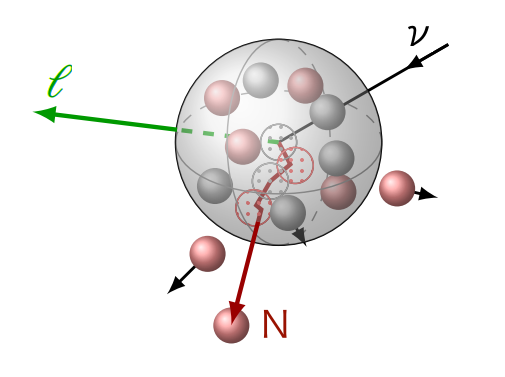
\includegraphics[width=\textwidth]{TalkPics/CorrelationWorkshop050217/interactionmodel.png}
    \end{columns}
  \end{frame}

  \begin{frame}
    \frametitle{What problems could we have?}
    \begin{itemize}
    \item Different nuclei at near and far detector
    \end{itemize}
    
      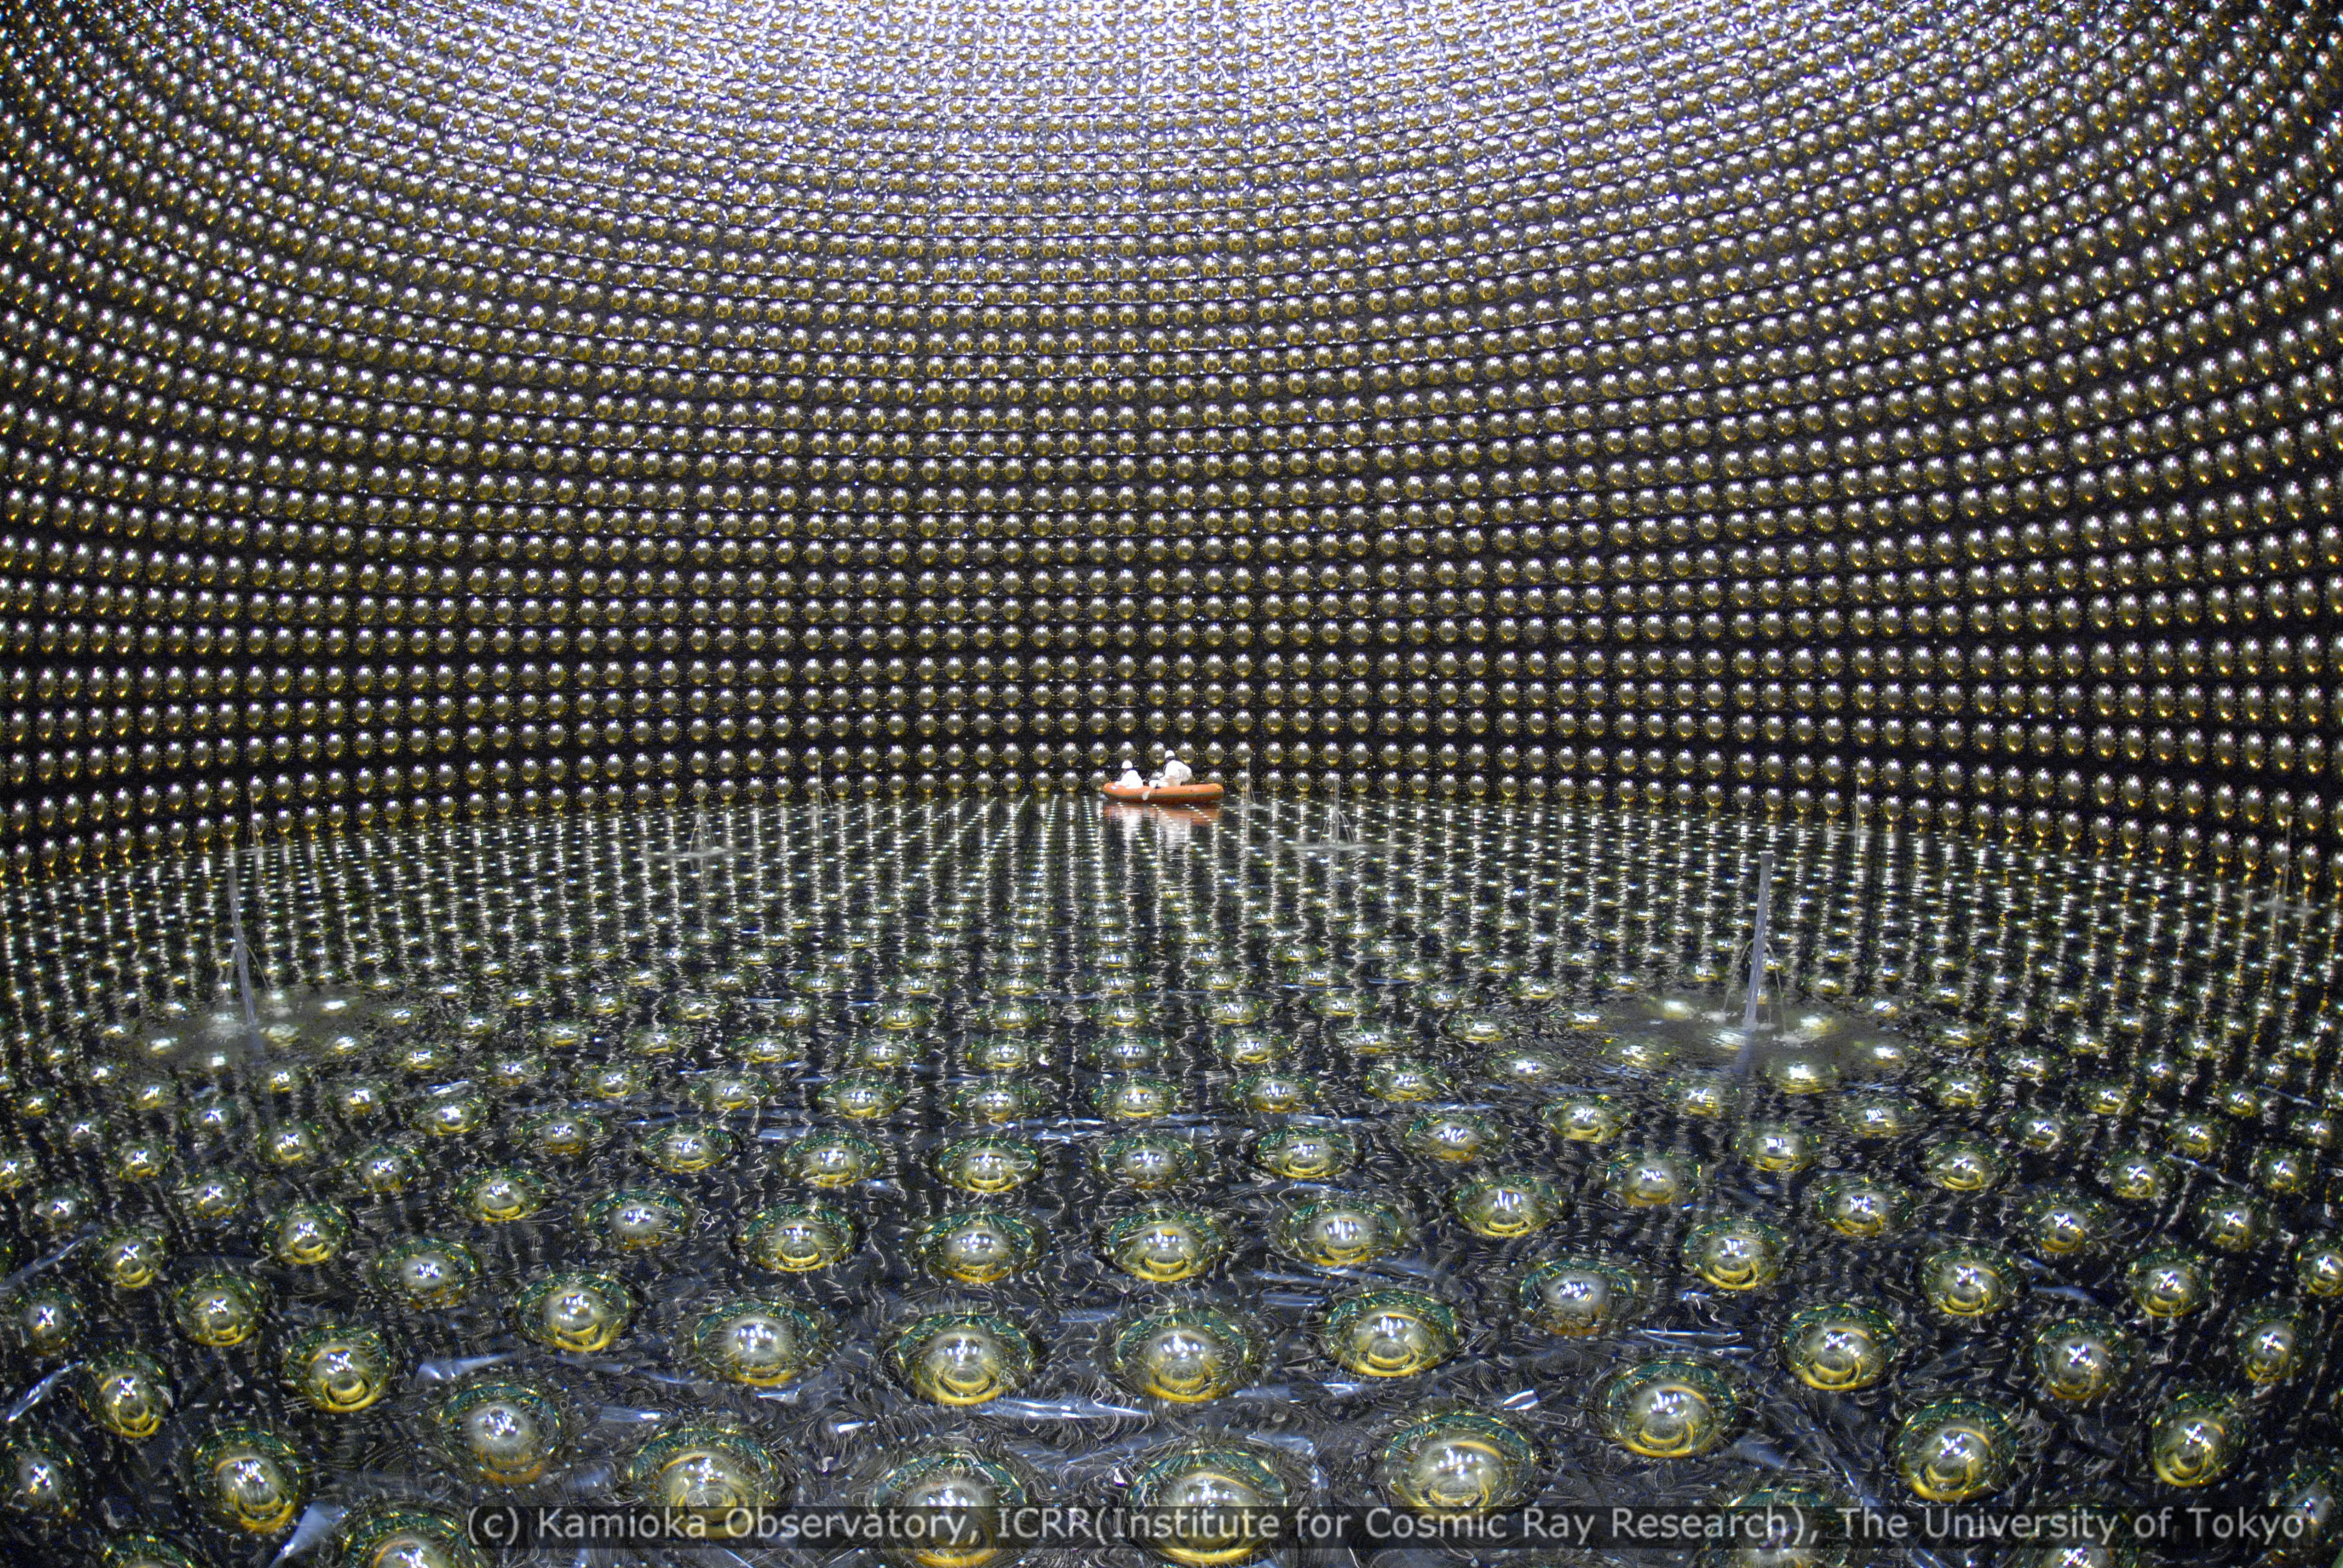
\includegraphics[width=.5\textwidth]{TalkPics/CorrelationWorkshop050217/SK.jpg}
      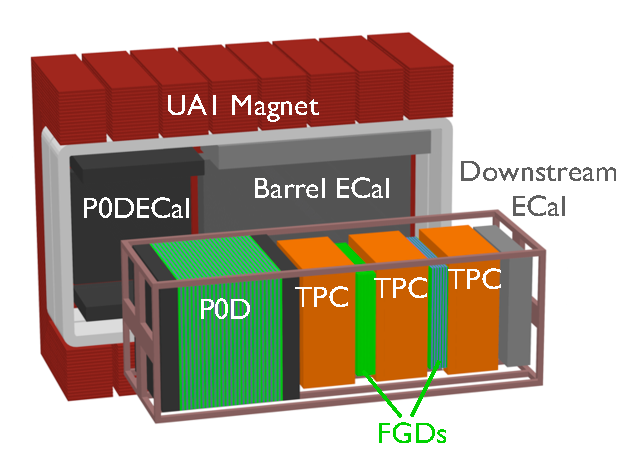
\includegraphics[width=.5\textwidth]{TalkPics/CorrelationWorkshop050217/nd280.png}

      \begin{itemize}
      \item Could use a water near detector like Nu-Prism/Titus
      \end{itemize}
  \end{frame}
  
  \begin{frame}
    \frametitle{What problems could we have?}
      \begin{itemize}
      \item Different energy spectrum at near and far detector
      \end{itemize}
      \centering
    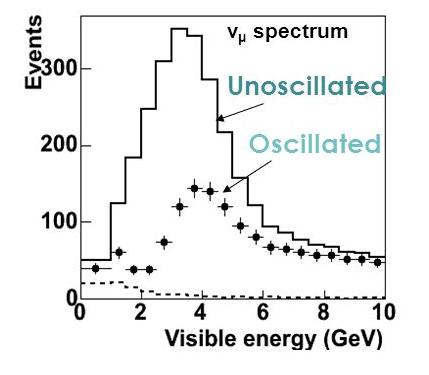
\includegraphics[width=.5\textwidth]{TalkPics/CorrelationWorkshop050217/oscunoscspectra.png}

    \begin{itemize}
    \item Even if same nucleus this can be problematic
    \end{itemize}
  \end{frame}

  \begin{frame}
    \frametitle{What can we do about it?}
    \begin{itemize}
    \item Great work already being done by xsec/external fitting groups
    \item Need to do more to test if $\nu/\bar{\nu}$ difference is from CP violation
    \item[-] Must look at more variables including hadronic ones
    \item[-] Must look at as many nuclei as possible
    \item Can use an HPTPC to do this
    \end{itemize}
  \end{frame}

  \begin{frame}
    \frametitle{What is an HPTPC?}
    \begin{itemize}
    \item Has the fine resolution and low thresholds of a TPC
    \item High pressure gives enough density to use as a target
    \item Can look at different nuclei by altering gas mix
    \end{itemize}
    \centering
    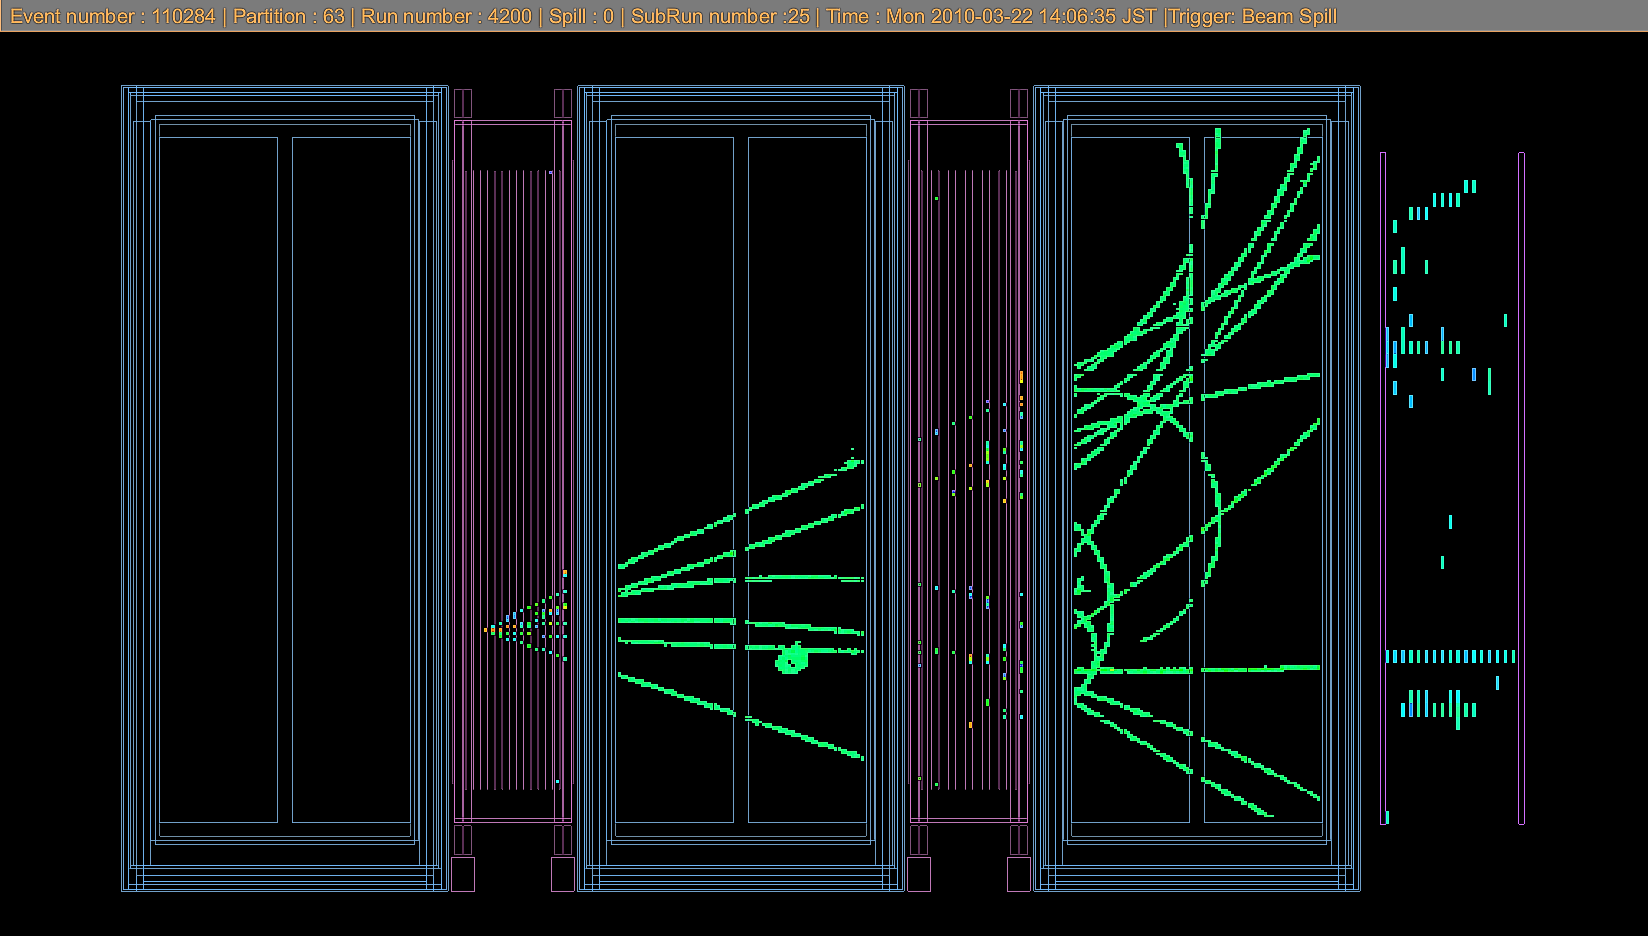
\includegraphics[width=.5\textwidth]{TalkPics/CorrelationWorkshop050217/nd280evdisp.png}
  \end{frame}

  \begin{frame}
    \frametitle{Sensitivity studies with HPTPC}
    \begin{itemize}
    \item Aim to include an $\sim$600kg HPTPC as an HK near detector
    \item Have taken ND280 truth MC and applied HPTPC like efficiencies and thresholds
    \item[-] Assumes same target nuclei as ND280
    \item Calculate event variables and compare detectors
    \item Low hadronic thresholds allow for use of hadron kinematics
    \end{itemize}
    \begin{tabular}{l|cc}
      \hline
      Particle & ND280 Threshold/MeV & HPTPC Threshold/MeV \\
      \hline
      $\mu$ & 100 & 15 \\
      $\pi$ & 120 & 16 \\
      $p$ & 450 & 60 \\
      $e$ & 100 & 1 \\
      \hline
    \end{tabular}
  \end{frame}

  %??what can we do with this hadron information STV
  \begin{frame}%??add more intro
    \frametitle{Single Transverse Variables}
    \vspace{-.3cm}
    \begin{itemize}
    \item Use hadronic information to estimate nuclear effects
    \item Any imbalance perpendicular to neutrino direction should come from nuclei/unseen particles
    \item[-] Details in Xianguo's talk
    \item Variables widely used in other areas of particle physics
    \end{itemize}
    \vspace{-.1cm}
    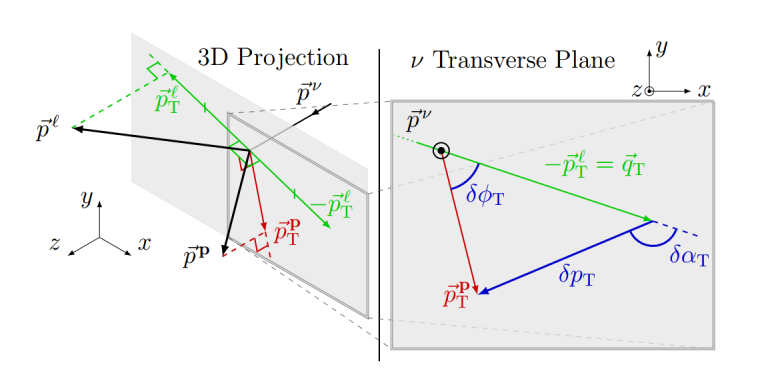
\includegraphics[width=\textwidth,clip=true,trim=0 0 0 20]{TalkPics/STVforHPTPC_101016/stvdiagram.png}
  \end{frame}

  \begin{frame}
    \frametitle{Aside on naming for STV}
    \begin{itemize}
    \item Naming that is emerging in neutrino physics is different from other areas: e.g. hadron colliders
    \scriptsize\item[-] $\delta p_{T}=p_{T}^{miss}$, $\delta\phi_{T}=\pi-\Delta\phi(lep,had)$, $\delta\alpha_{T}=\pi-\Delta\phi(lep,p_{T}^{miss})$
    \normalsize
    \item Personally find hadron collider naming more intuitive
    \item Worth considering whether we want to standardise
    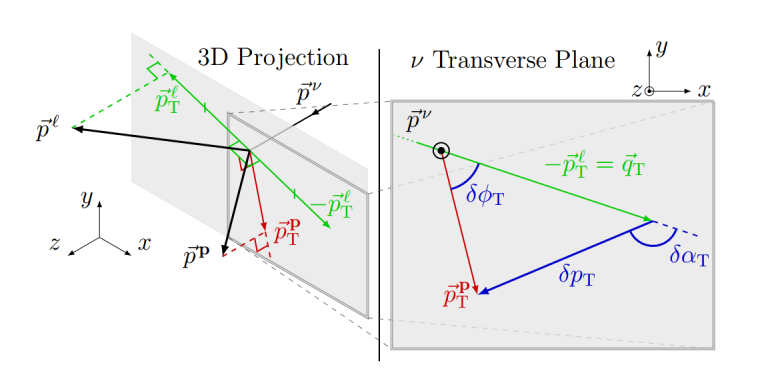
\includegraphics[width=\textwidth,clip=true,trim=0 0 0 20]{TalkPics/STVforHPTPC_101016/stvdiagram.png}
    \end{itemize}
  \end{frame}

  \begin{frame}
    \frametitle{1D distributions for CC0$\pi$1p}
    \centering
    \begin{itemize}
    \item Use truth information to separate correctly identified real CC0$\pi$1p events from fakes
    \item HPTPC event rates are lower but purity is much better
    \end{itemize}
    \centering
    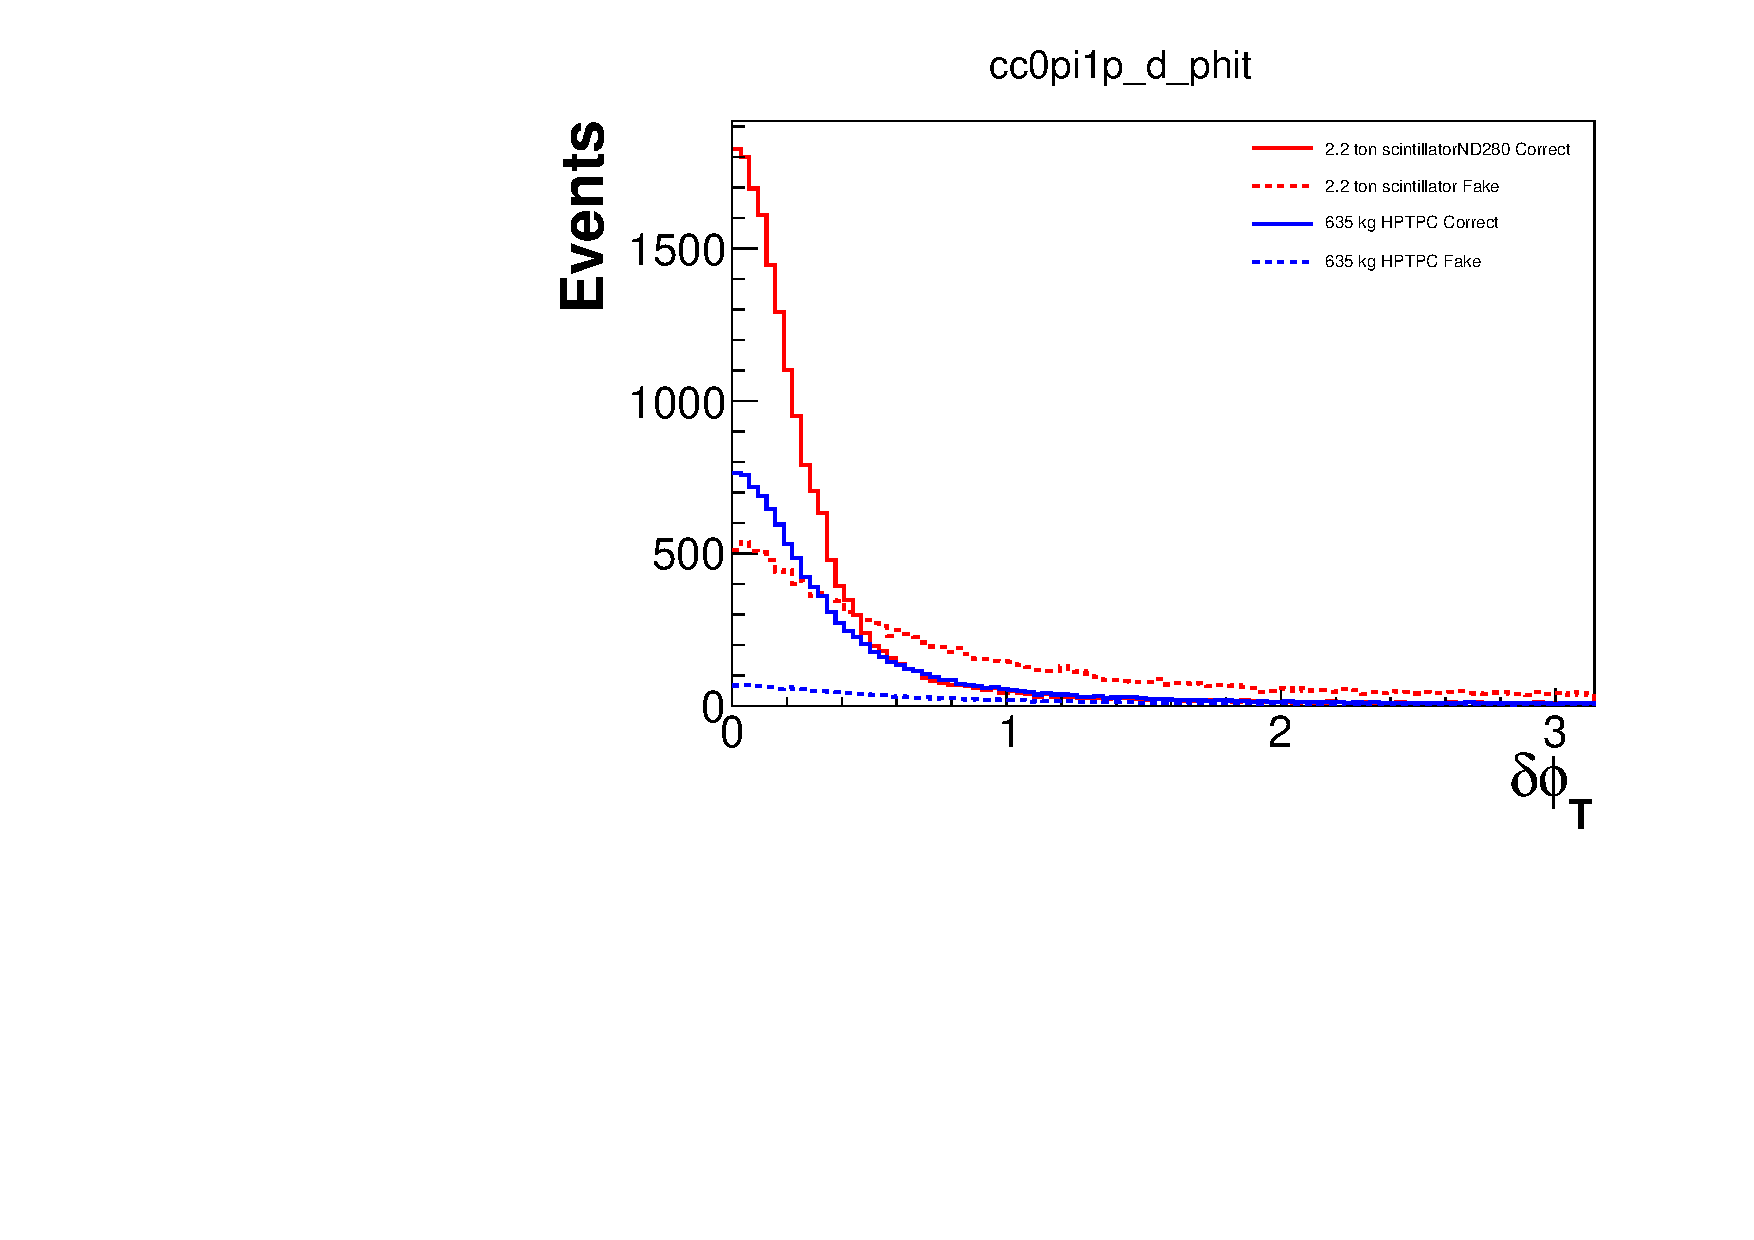
\includegraphics[width=.7\textwidth]{TalkPics/STVforHPTPC_211116/hptpcplots_211116/cc0pi1p_d_phit.pdf}
  \end{frame}

  \begin{frame}
    \frametitle{1D distributions for CC0$\pi$1P}
    \begin{itemize}
    \item Shape differences with nominal model aren't that great
    \item But aim is not just to add samples to BANFF fit
    \end{itemize}
    \centering
    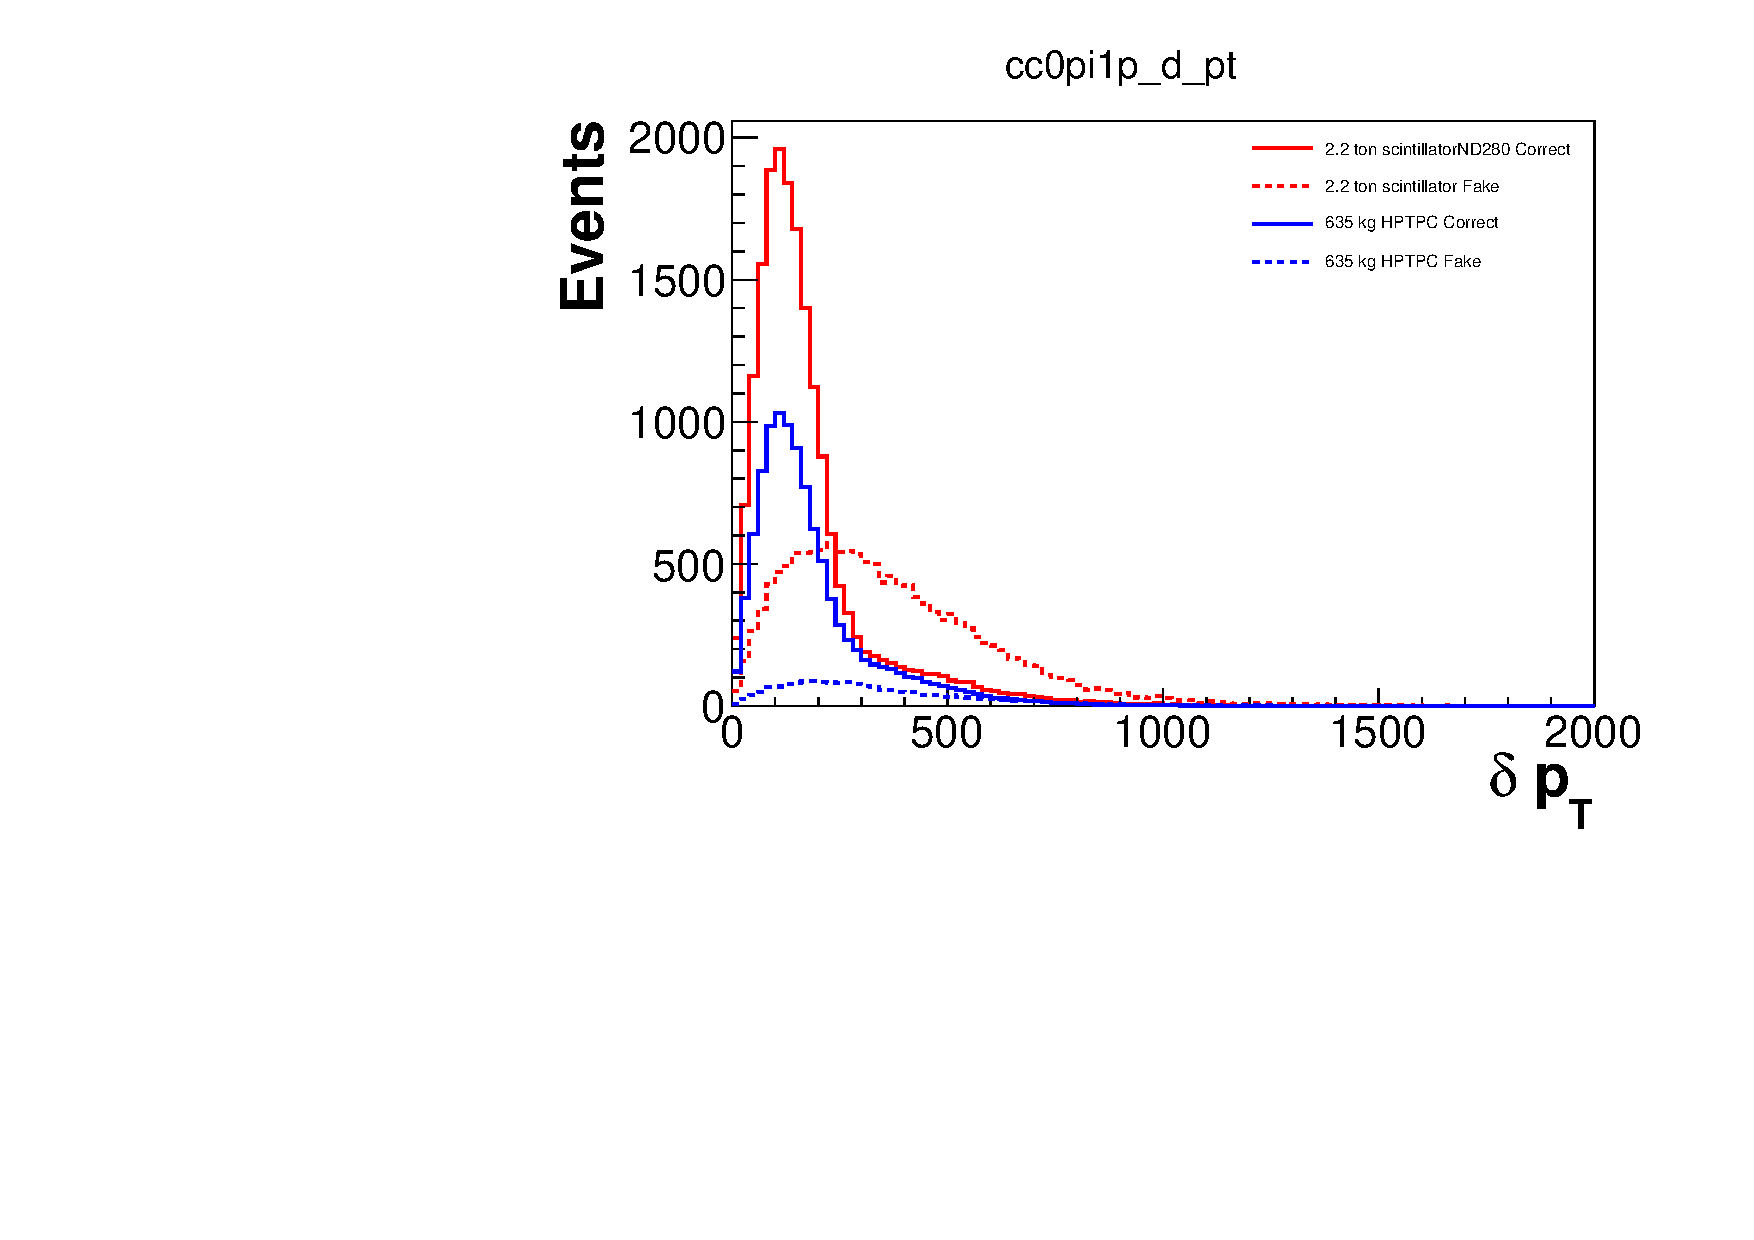
\includegraphics[width=.7\textwidth]{TalkPics/STVforHPTPC_211116/hptpcplots_211116/cc0pi1p_d_pt.pdf}
  \end{frame}

  \begin{frame}
    \frametitle{1D distributions for CC0$\pi$1P}
    \begin{itemize}
    \item Hope to use HPTPC for model selection
    \item High purity sample can be reliably compared to MC
    \end{itemize}
    \centering
    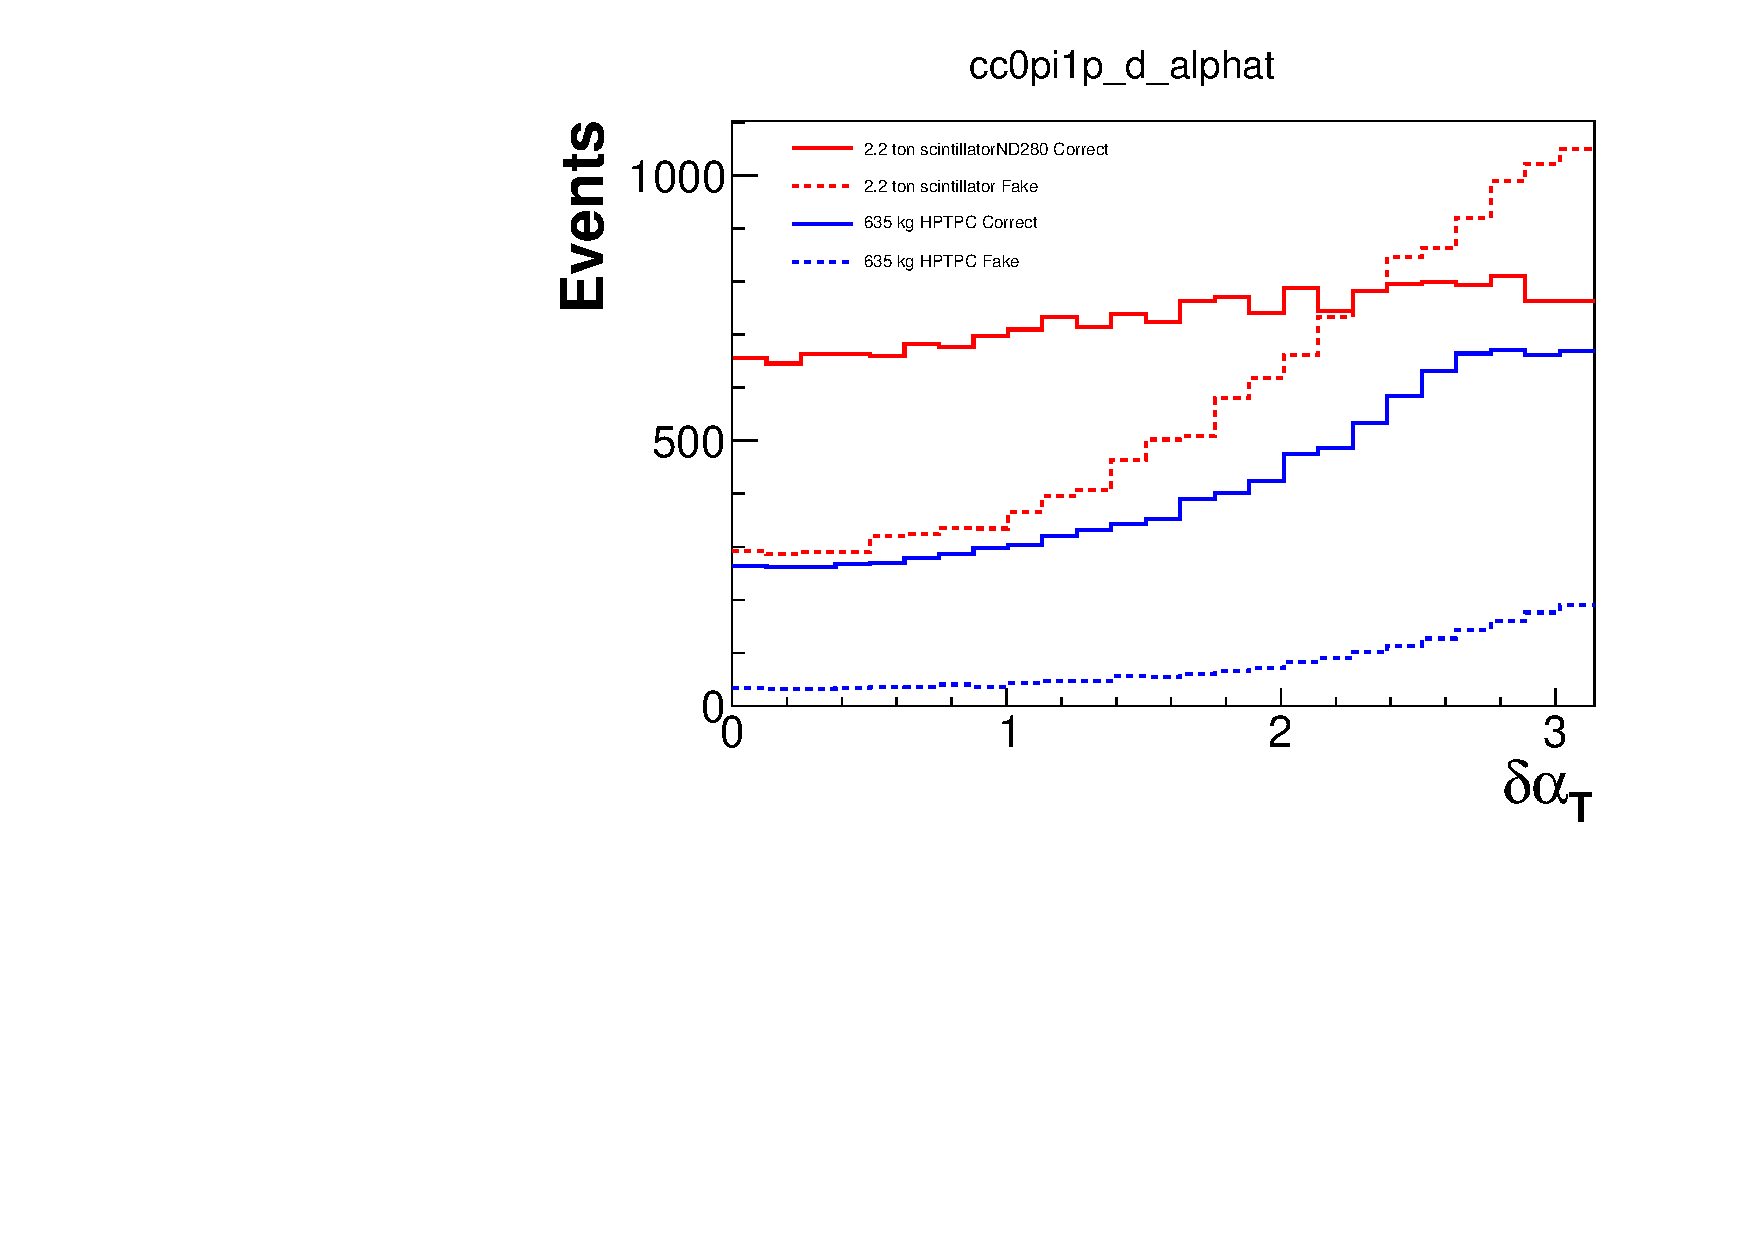
\includegraphics[width=.7\textwidth]{TalkPics/STVforHPTPC_211116/hptpcplots_211116/cc0pi1p_d_alphat.pdf}
  \end{frame}

  \begin{frame}
    \frametitle{2D distributions for CC0$\pi$1P}
    \begin{itemize}
    \item Also look at 2D distributions
    \end{itemize}
    \centering
    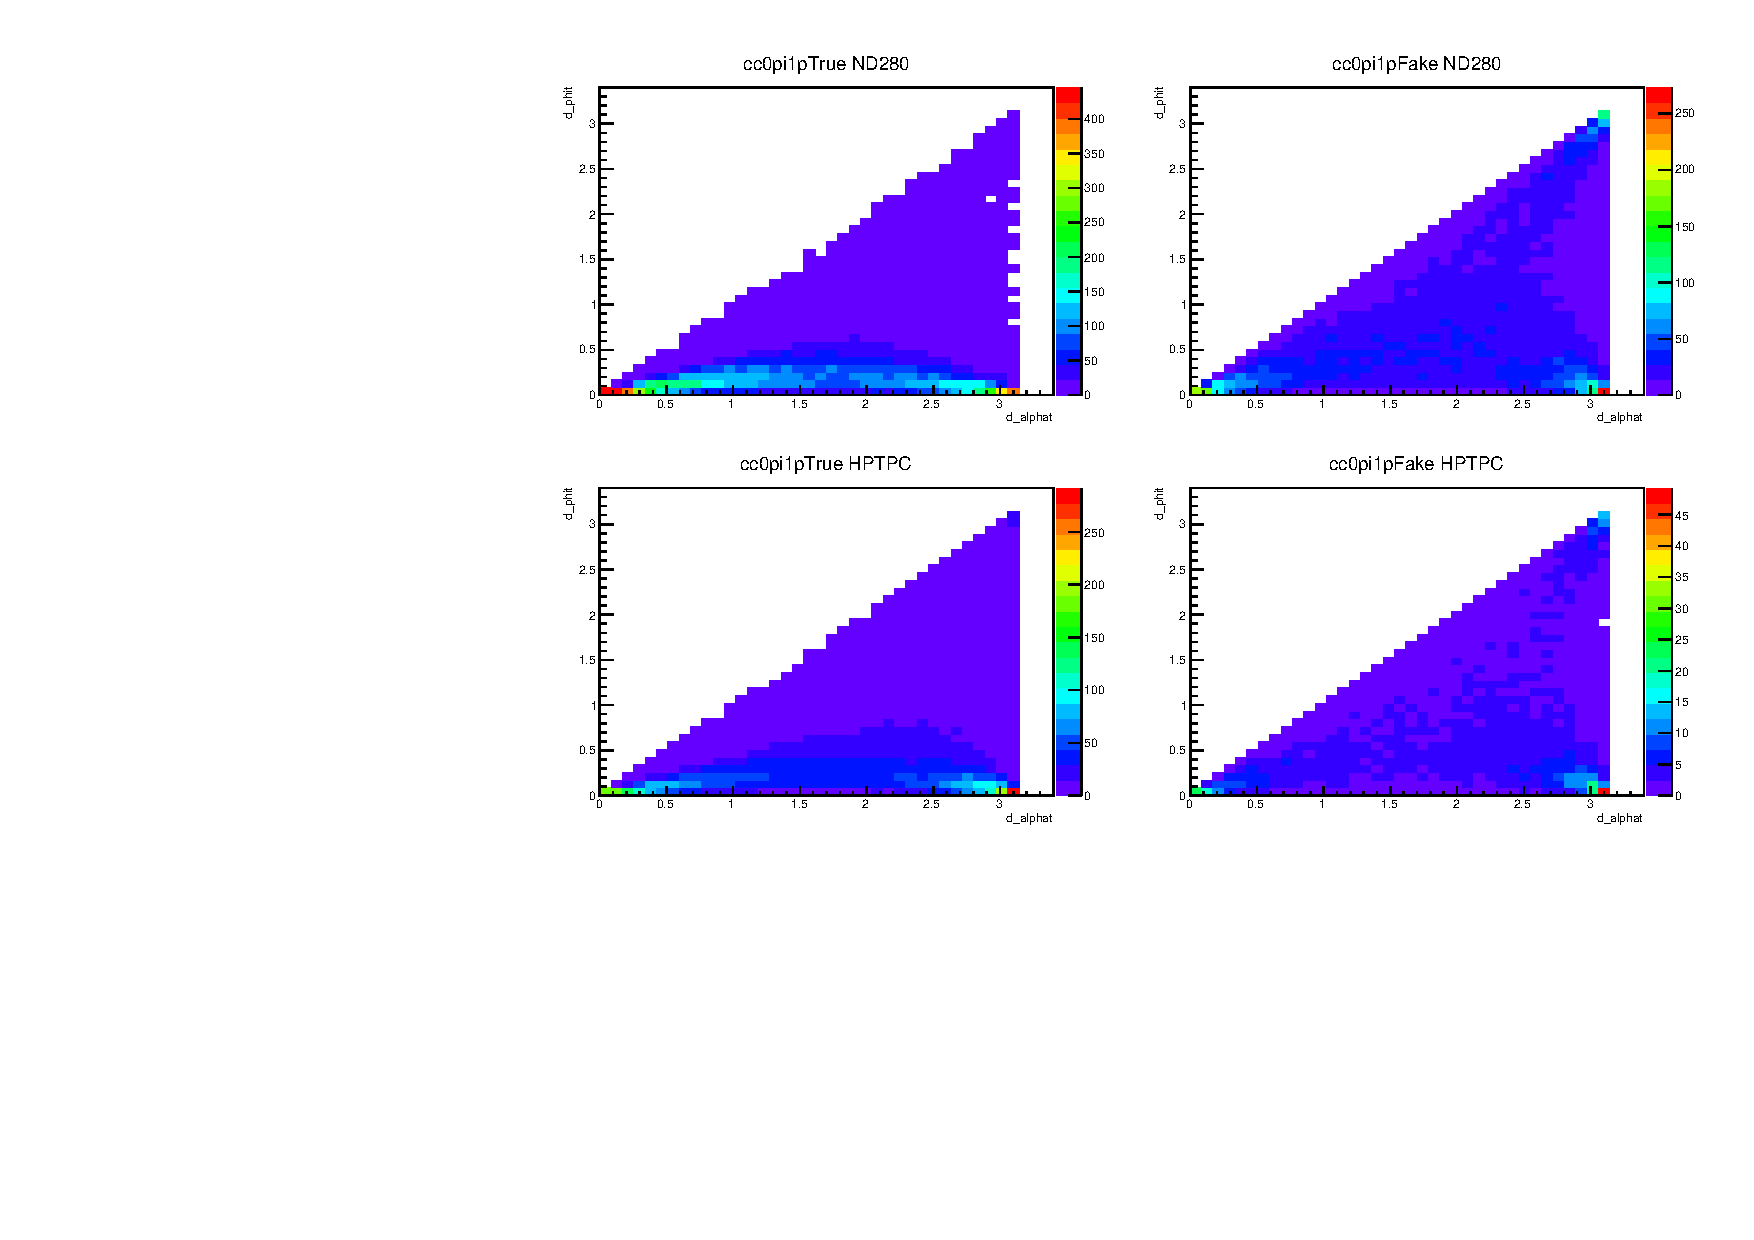
\includegraphics[width=.8\textwidth]{TalkPics/STVforHPTPC_211116/hptpcplots_211116/cc0pi1p_d_phitd_alphat.pdf}
  \end{frame}

  \begin{frame}
    \frametitle{2D distributions for CC0$\pi$1P}
    \begin{itemize}
    \item And compare lepton and hadron variables
    \end{itemize}
    \centering
    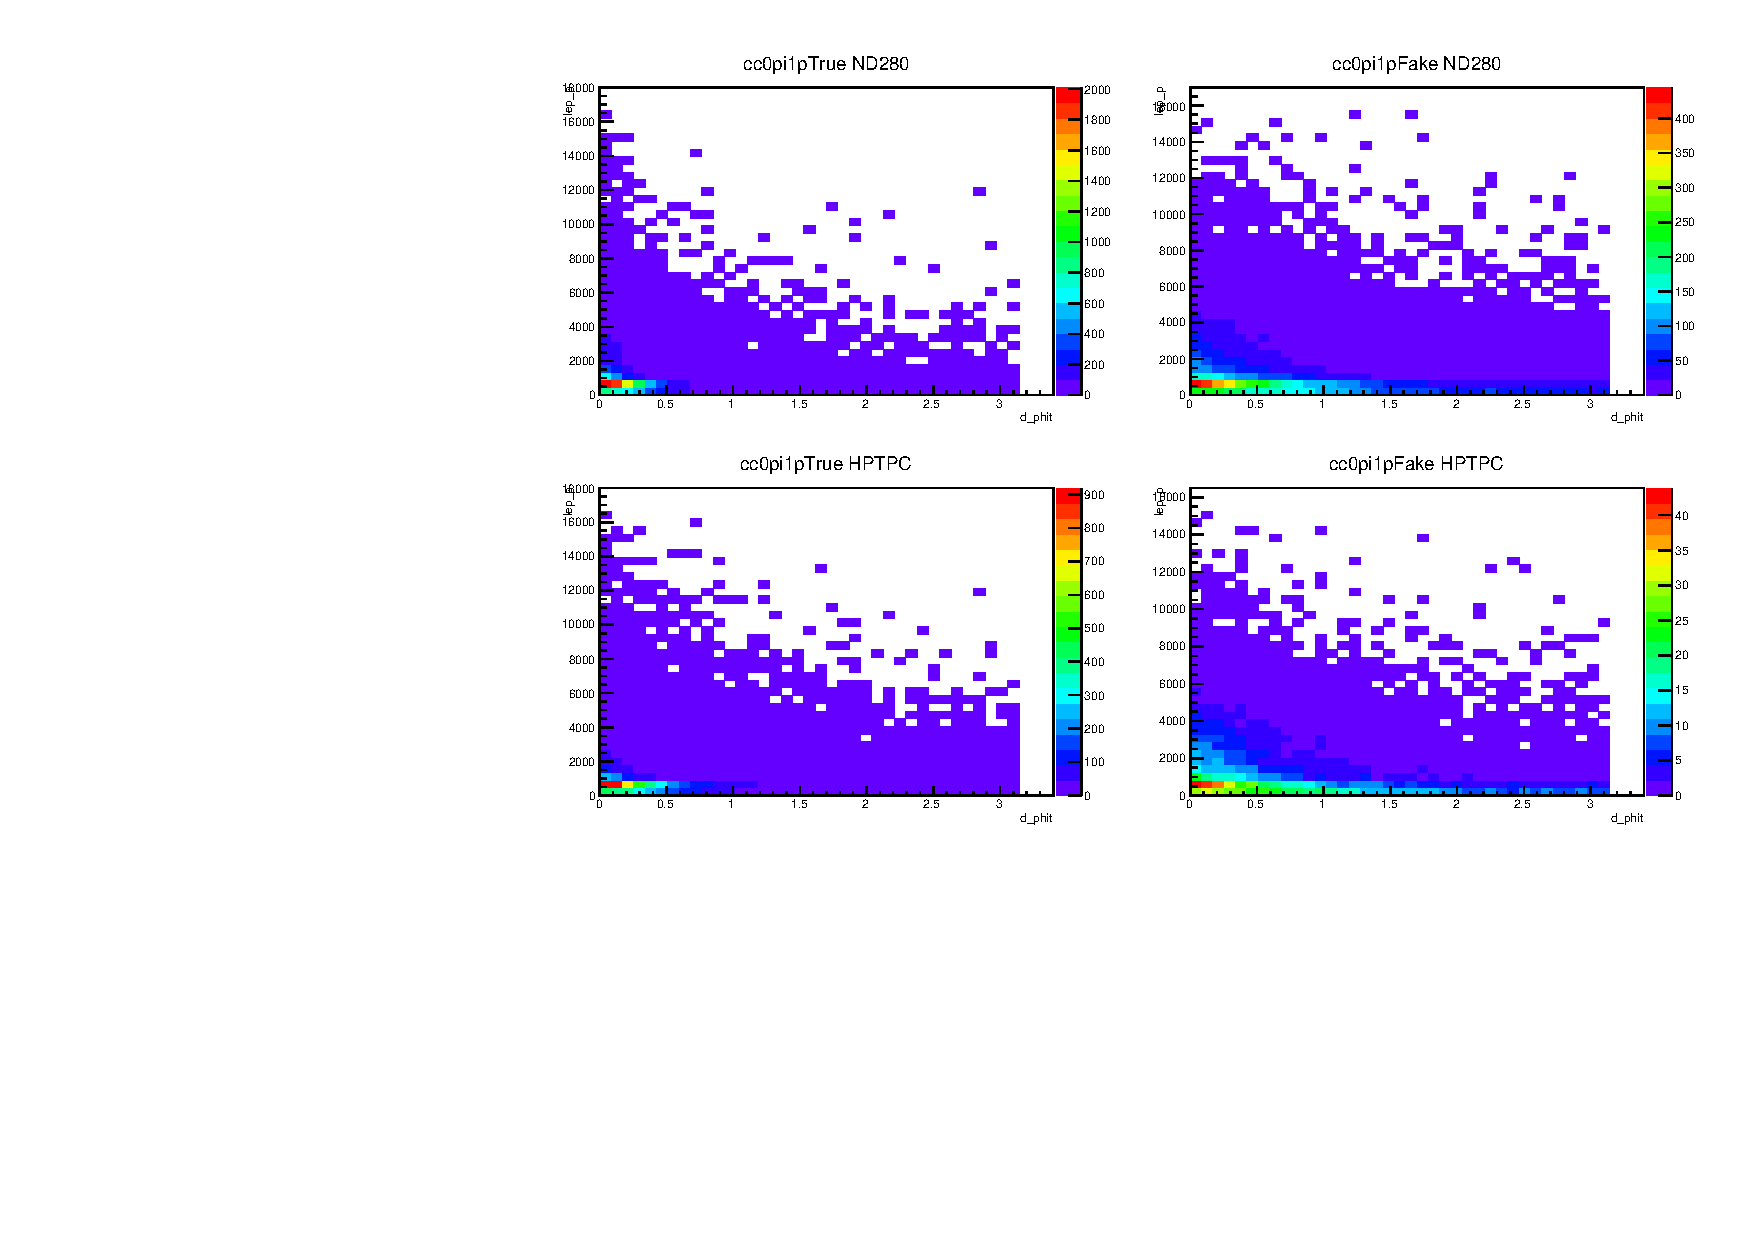
\includegraphics[width=.8\textwidth]{TalkPics/STVforHPTPC_211116/hptpcplots_211116/cc0pi1p_lep_pd_phit.pdf}
  \end{frame}


  %??more info
  \begin{frame}
    \frametitle{Other Transverse Variables - Reminder}
    \begin{itemize}
    \item Particularly for $p_{T}^{miss}$ context is important
    \end{itemize}
    \begin{block}{}
      \centering
      \begin{fmfgraph*}(60,50)
        \fmftop{i1,m1,m2,m3,m4,m5,m6,m7,o1}
        \fmfbottom{i2,m8,m9,m10,m11,o2}
        \fmf{fermion,tension=4}{v1,i2}
        \fmf{fermion,tension=4}{v1,o2}
        \fmf{fermion}{v1,m1}
        \fmf{dashes}{v1,m3}
        \fmf{fermion}{v1,m4}
        \fmf{fermion}{v1,m5}
        \fmf{fermion}{v1,m6}
        \fmf{fermion}{v1,m7}
        \fmf{fermion}{v1,m8}
        \fmf{fermion}{v1,m9}
        \fmf{fermion}{v1,m10}
        \fmf{fermion}{v1,m11}
      \end{fmfgraph*}
      \hspace{1.5cm}
      VS
      \hspace{1.5cm}
      \begin{fmfgraph*}(60,50)
        \fmftop{i1,m1,m2,m3,m4,m5,m6,m7,o1}
        \fmfbottom{i2,m8,m9,m10,m11,o2}
        \fmf{fermion,tension=4}{v1,i2}
        \fmf{fermion,tension=4}{v1,o2}
        \fmf{fermion}{v1,m1}
        \fmf{dashes}{v1,m3}
      \end{fmfgraph*}
      \vspace{.2cm}
    \end{block}
    \begin{itemize}
    \item Both events have the same $p_{T}^{miss}/\delta p_{T}$ but on the right this is clearly more significant compared to uncertainties on visible object momenta
    \end{itemize}
    
  \end{frame}

  %??show other variables results
  \begin{frame}
    \frametitle{Additional information}
    \begin{itemize}
      \item Look at component of proton momentum in transverse plane
    \end{itemize}
    \centering
    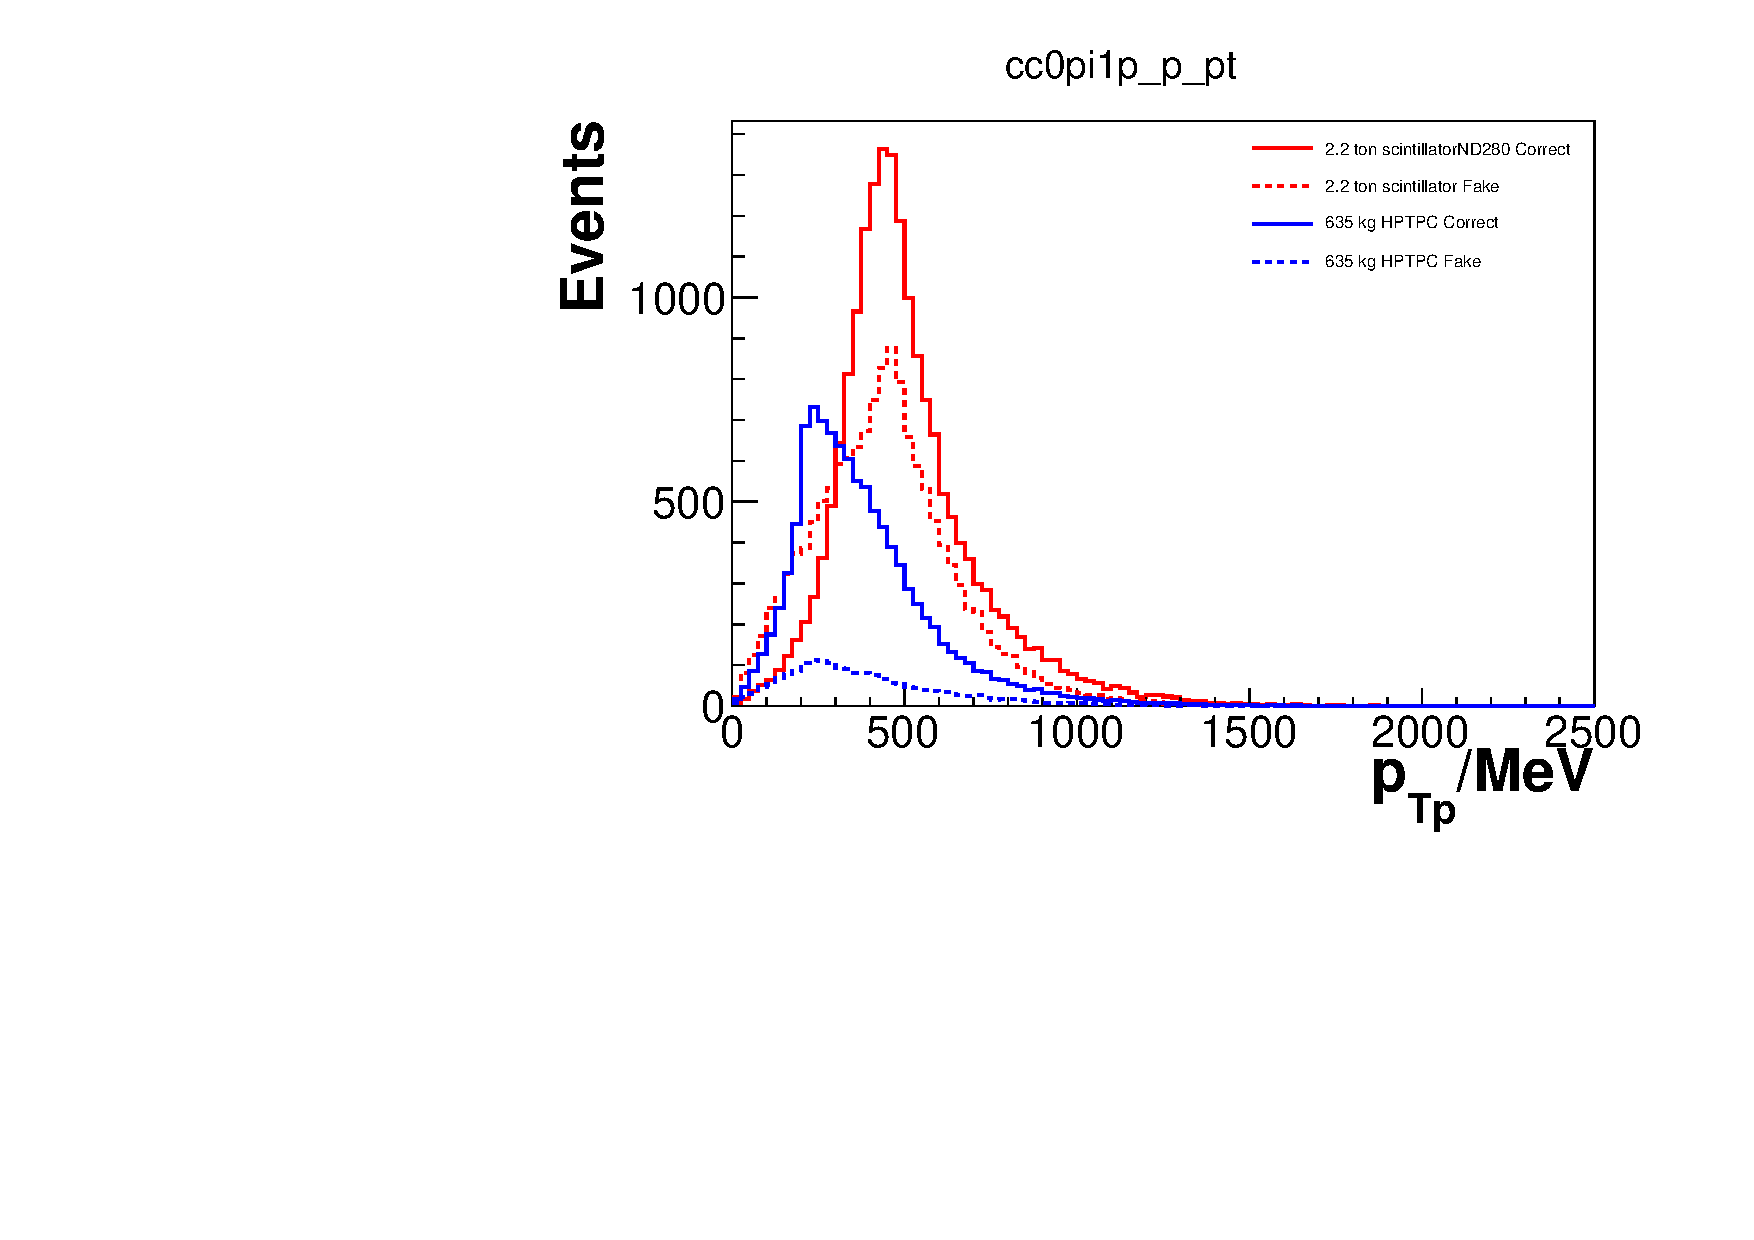
\includegraphics[width=.7\textwidth]{TalkPics/STVforHPTPC_211116/hptpcplots_211116/cc0pi1p_p_pt.pdf}
  \end{frame}

  \begin{frame}
    \frametitle{2D distribution highlights for CC0$\pi$1P}
    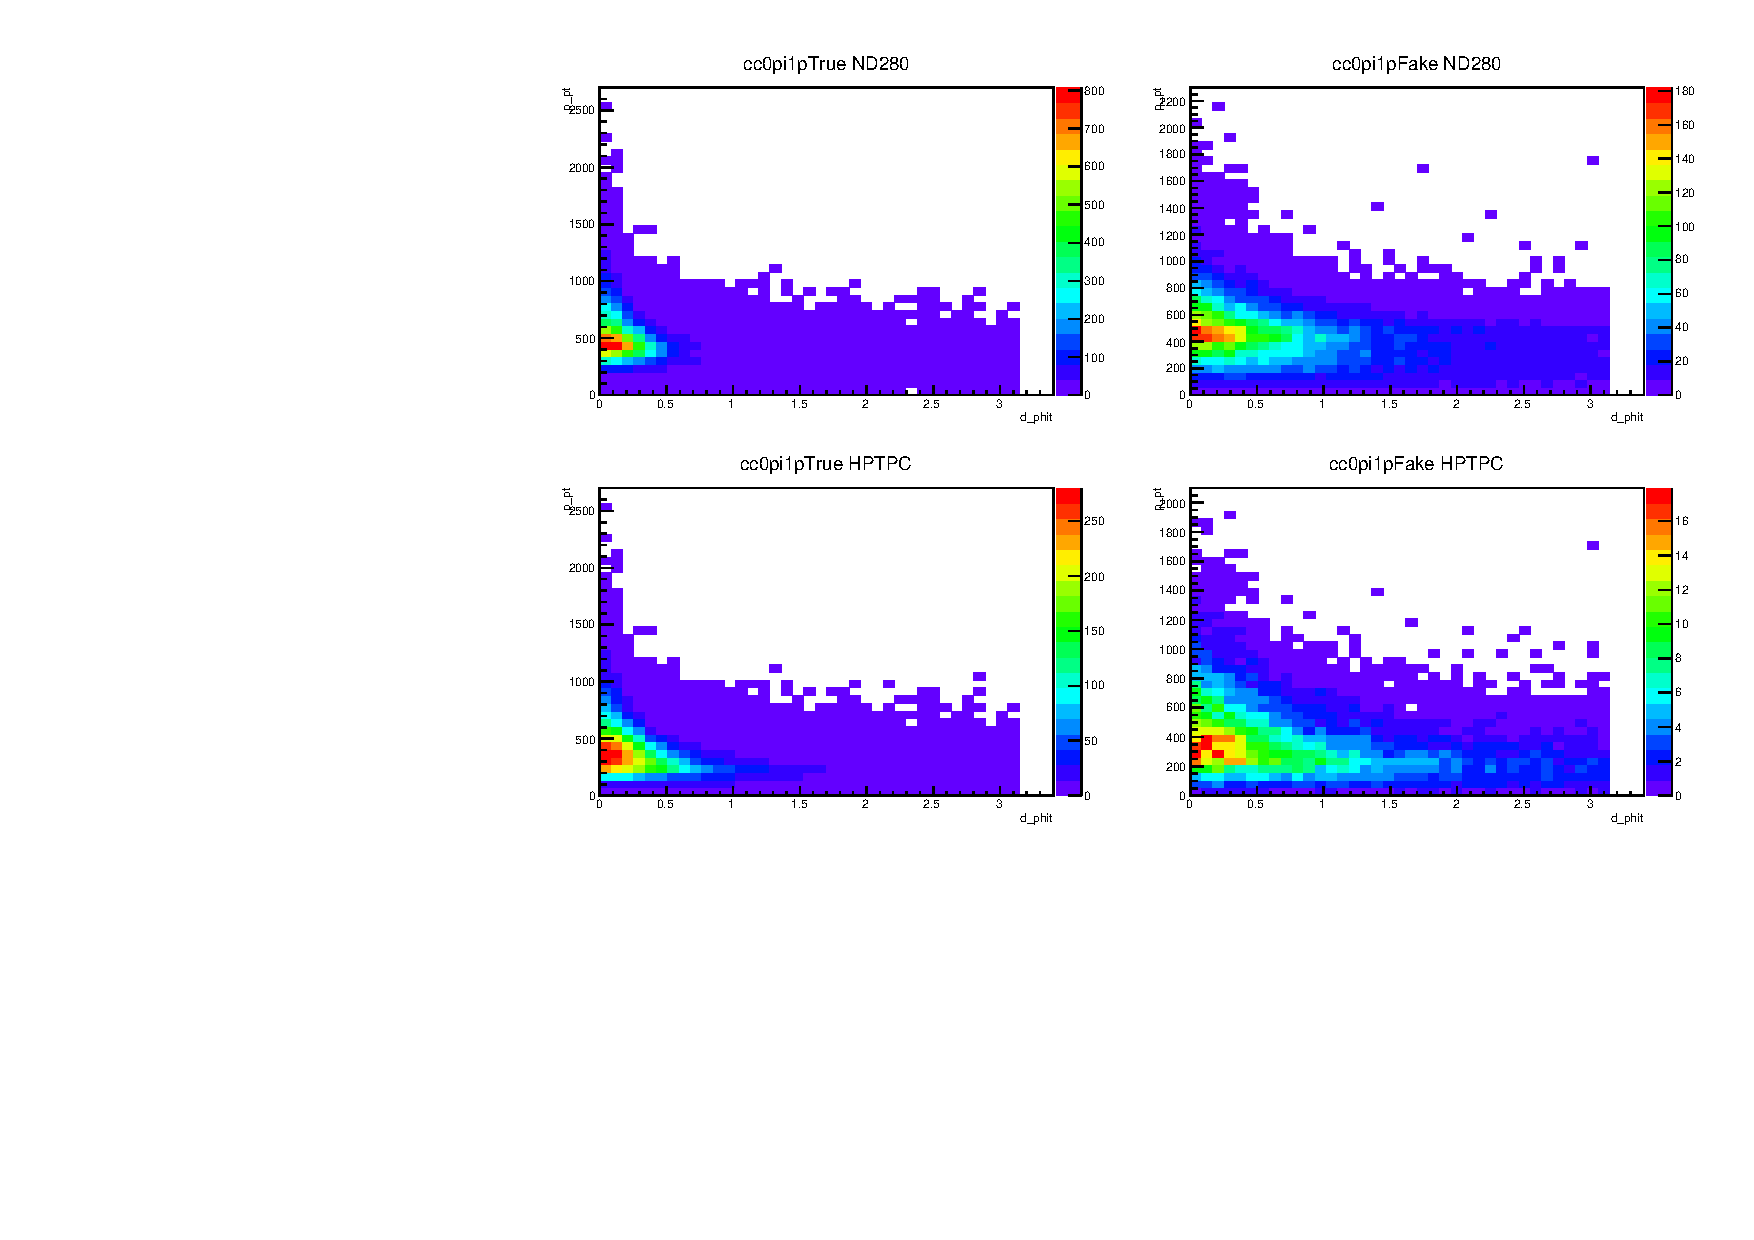
\includegraphics[width=.9\textwidth]{TalkPics/STVforHPTPC_211116/hptpcplots_211116/cc0pi1p_p_ptd_phit.pdf}
  \end{frame}

  \begin{frame}
    \frametitle{2D distribution highlights for CC0$\pi$1P}
    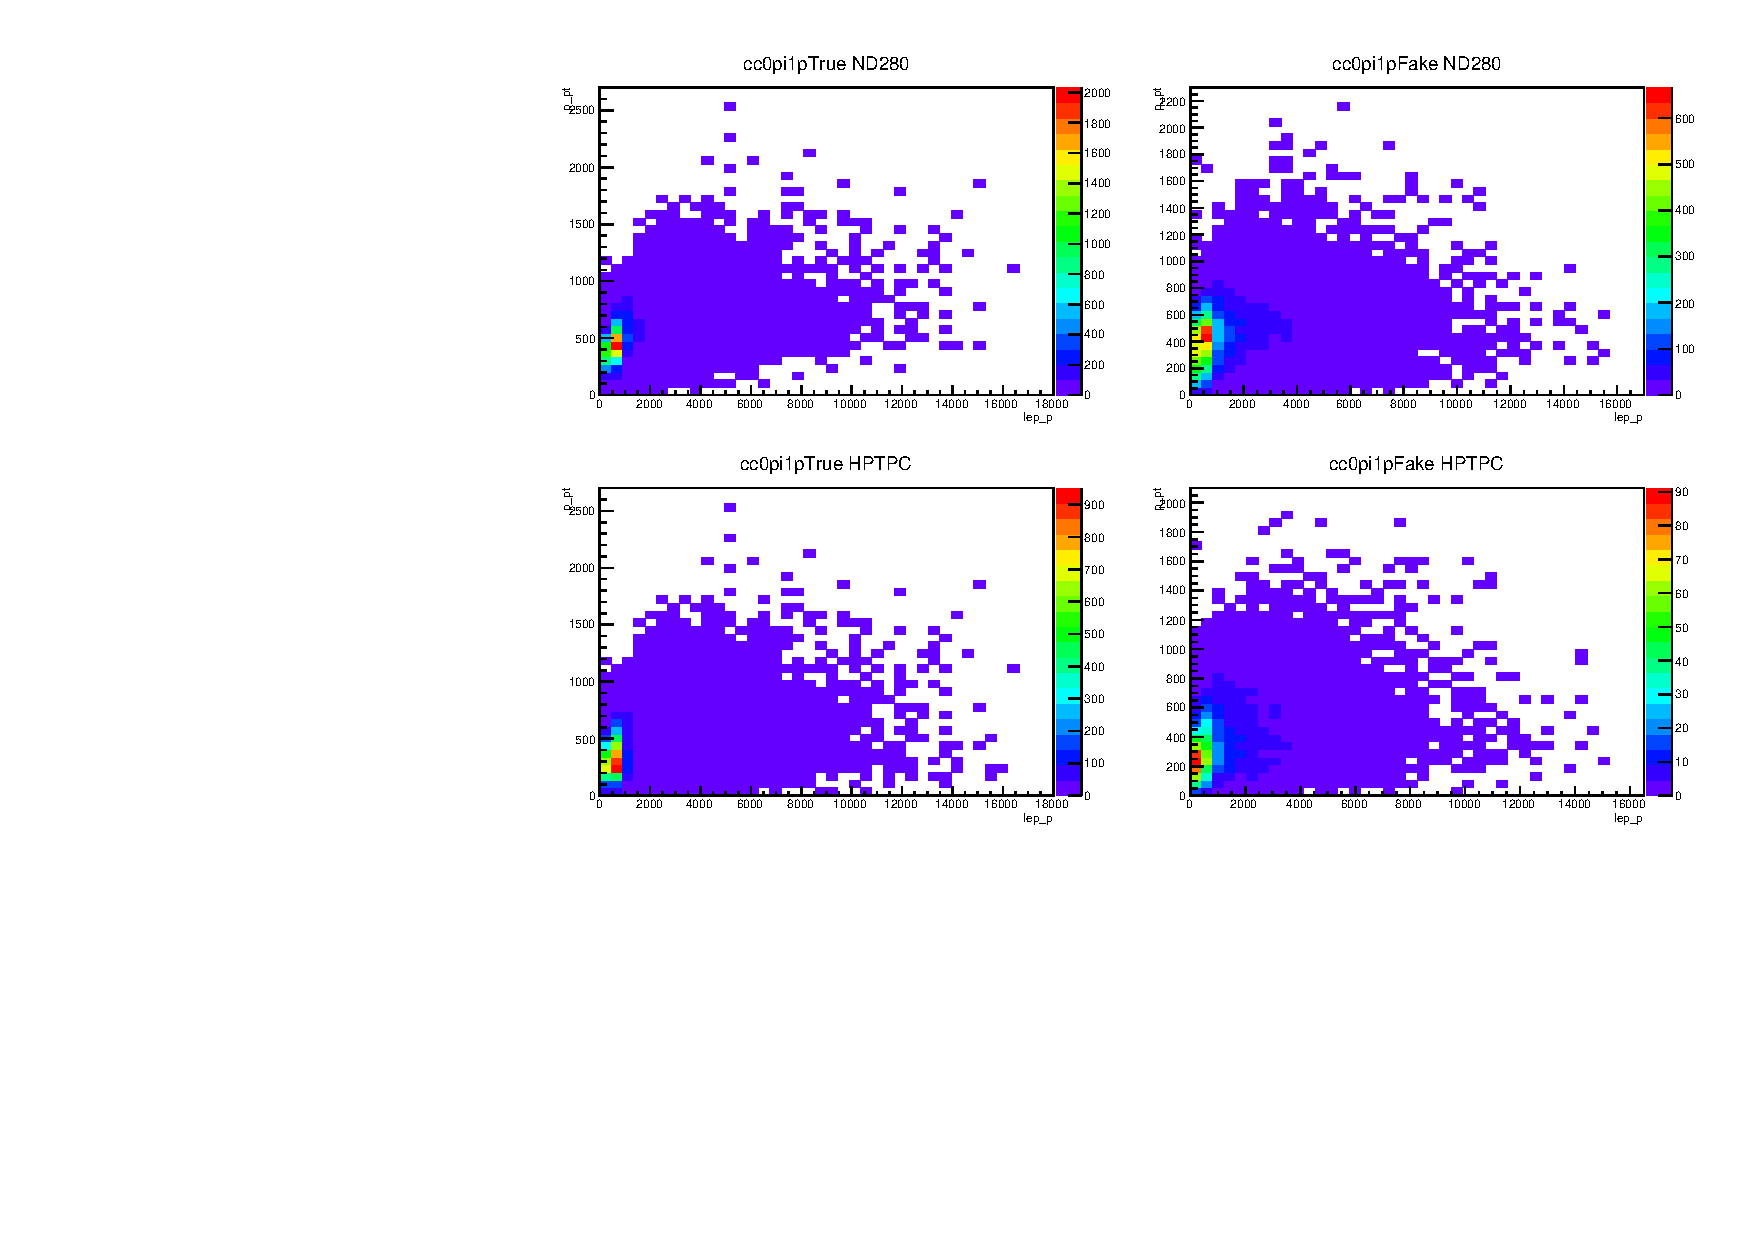
\includegraphics[width=.9\textwidth]{TalkPics/STVforHPTPC_211116/hptpcplots_211116/cc0pi1p_p_ptlep_p.pdf}
  \end{frame}

  \begin{frame}
    \frametitle{Model selection}
    \begin{itemize}
    \item Have studied HPTPC ability to discriminate between 2p2h models
    \item 2p2h Describes interactions between neutrino and 2 nucleons
    \item MC is generated with Nieves model
    \item Existing fake data studies use reweighting to study Martini model
    \end{itemize}
  \end{frame}

  %??some plots for HPTPC and ND280 showing not much difference
  \begin{frame}
    \frametitle{CC0$\pi$1p - Martini/Nieves}
    \begin{itemize}
    \item Don't see that much sensitivity when looking at proton momentum
    \end{itemize}
    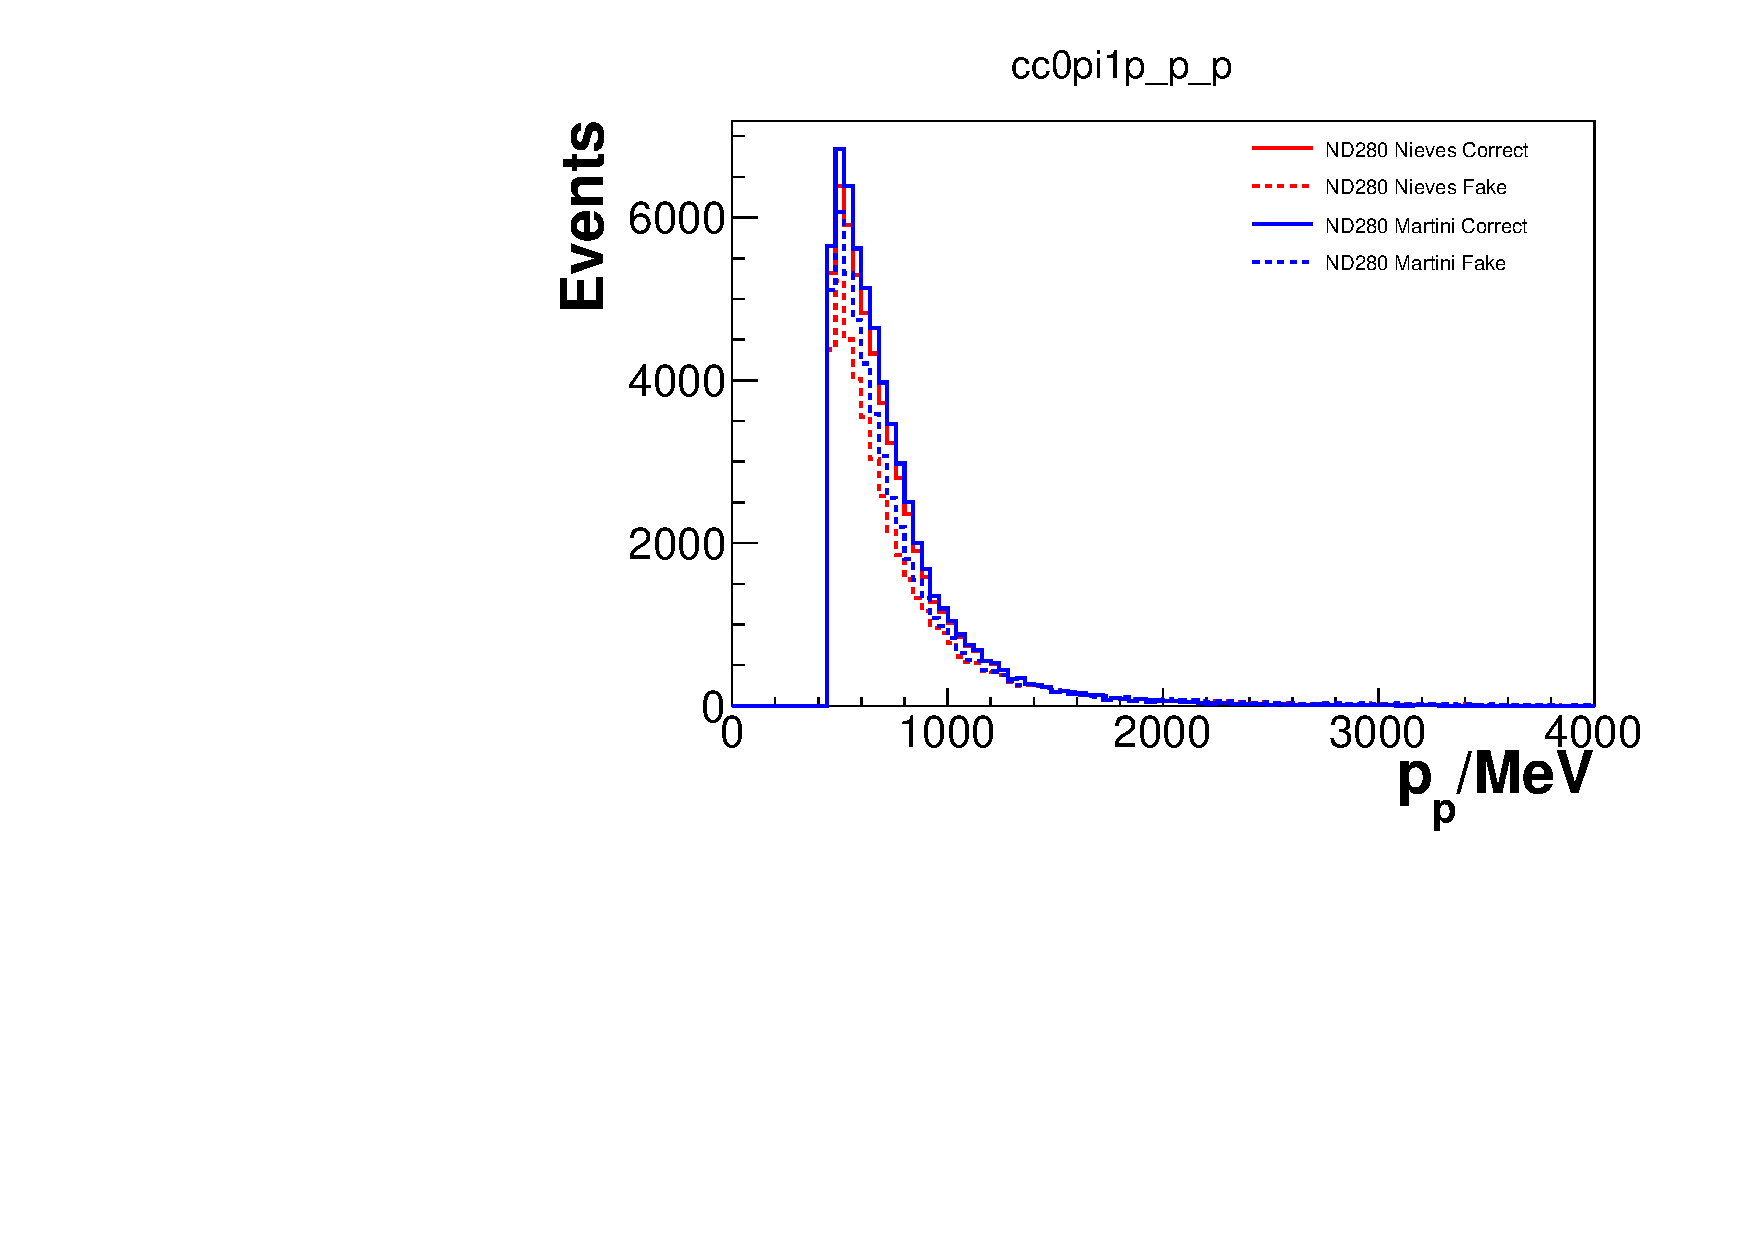
\includegraphics[width=.5\textwidth]{TalkPics/STVforHPTPC_191216/plots_martininievesnd280/cc0pi1p_p_p.pdf}
    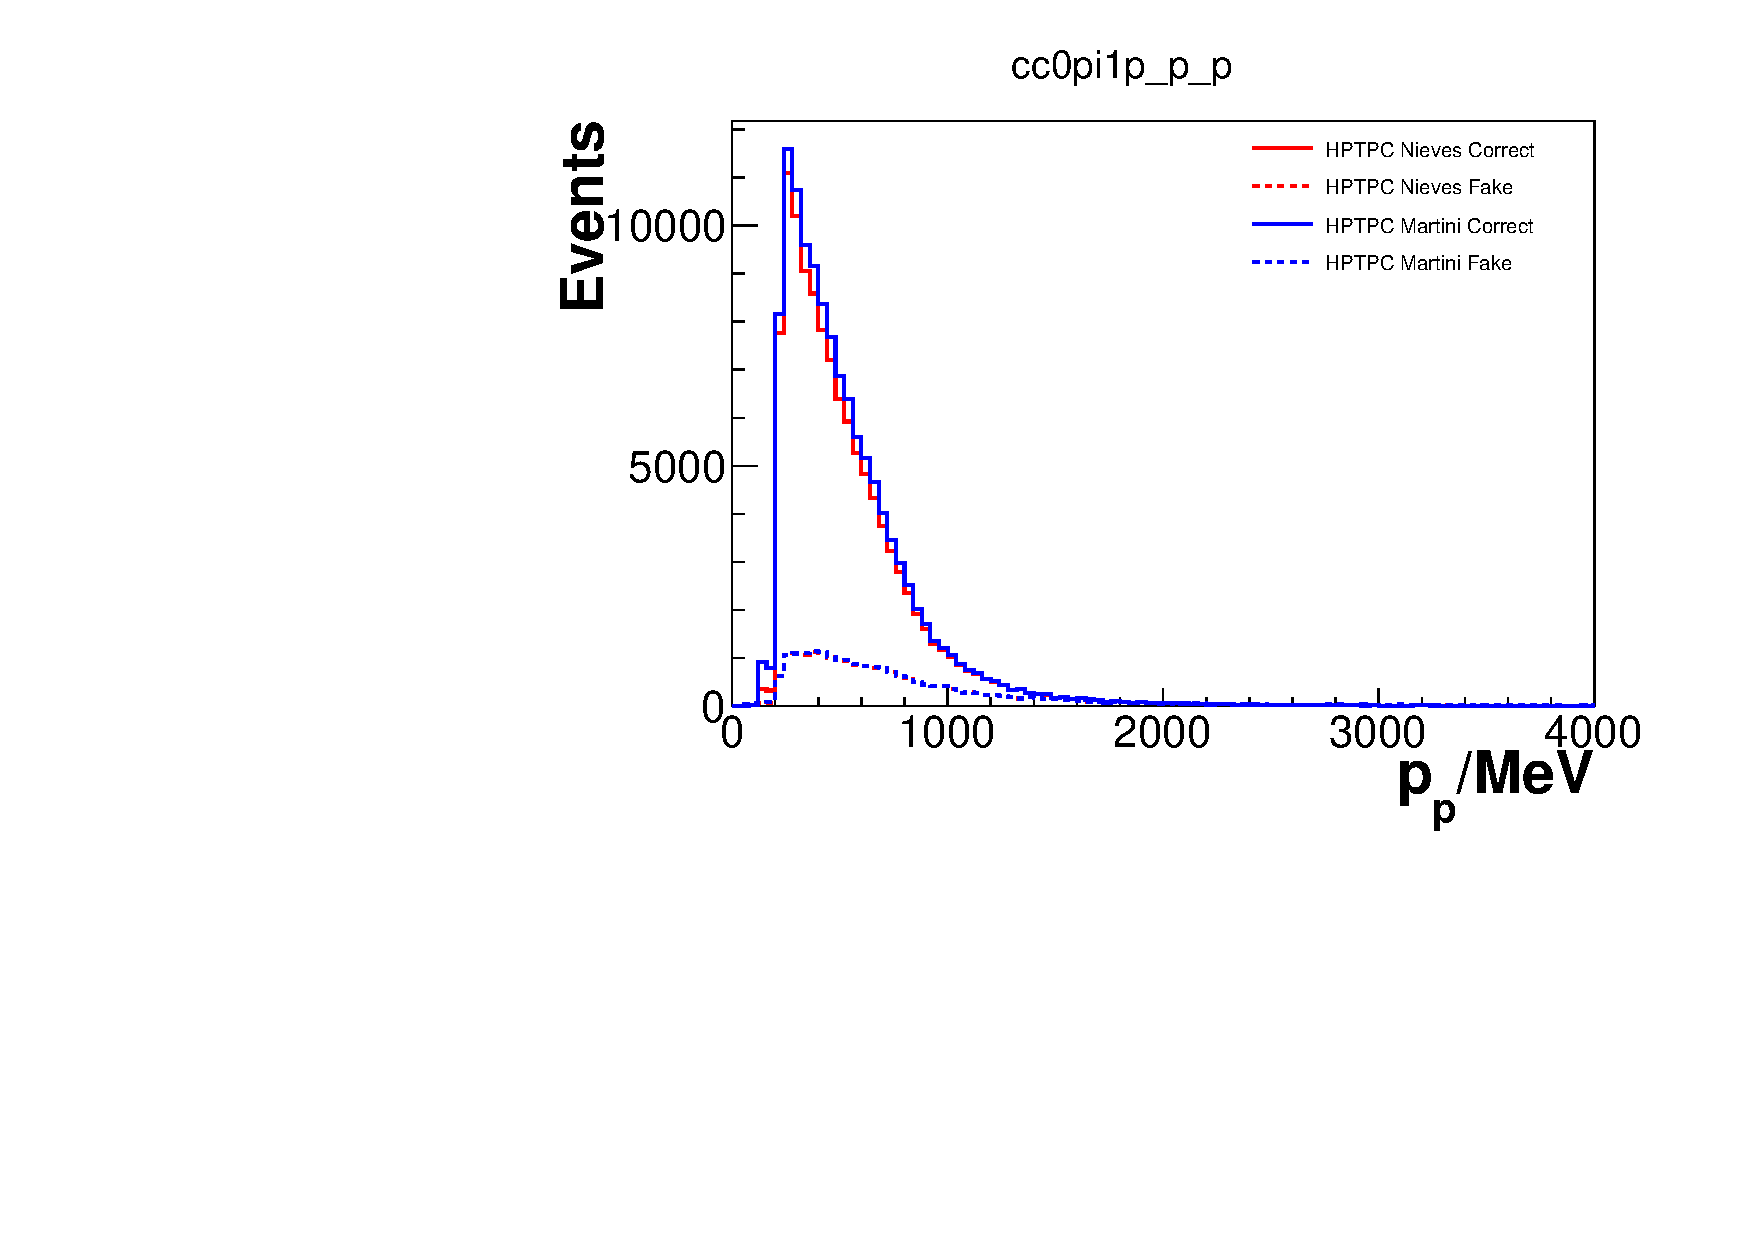
\includegraphics[width=.5\textwidth]{TalkPics/STVforHPTPC_191216/plots_martininieveshptpc/cc0pi1p_p_p.pdf}
  \end{frame}

  \begin{frame}
    \frametitle{CC0$\pi$1p - Martini/Nieves}
    \begin{itemize}
    \item Try `$p_{T}^{miss}$ significance' variable
    \item[-] Divide $p_{T}^{miss}$ by $\sqrt{p_{Tp}}$ 
    \item Provides good fake/correct discrimination
    \item Still not much model sensitivity
    \end{itemize}
    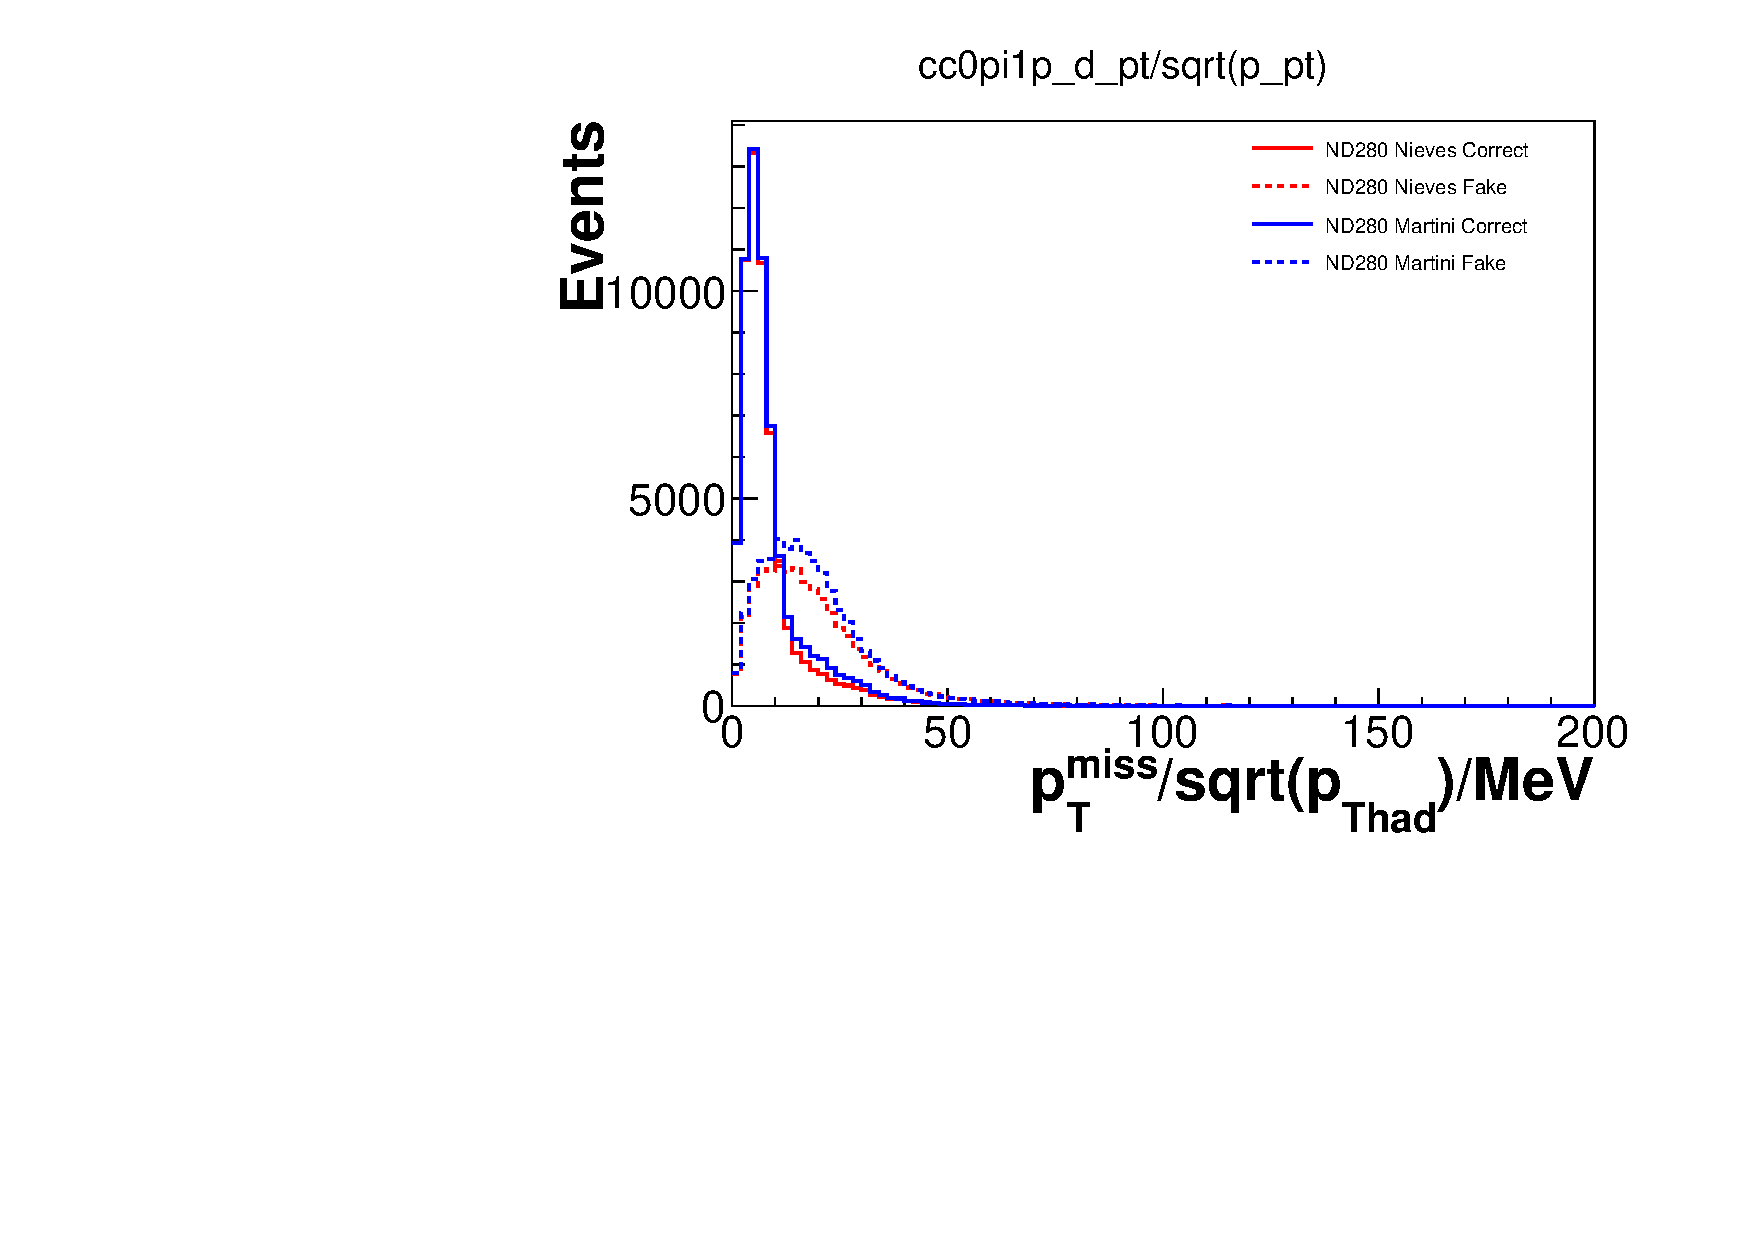
\includegraphics[width=.5\textwidth]{TalkPics/STVforHPTPC_191216/plots_martininievesnd280/cc0pi1p_metsig.pdf}
    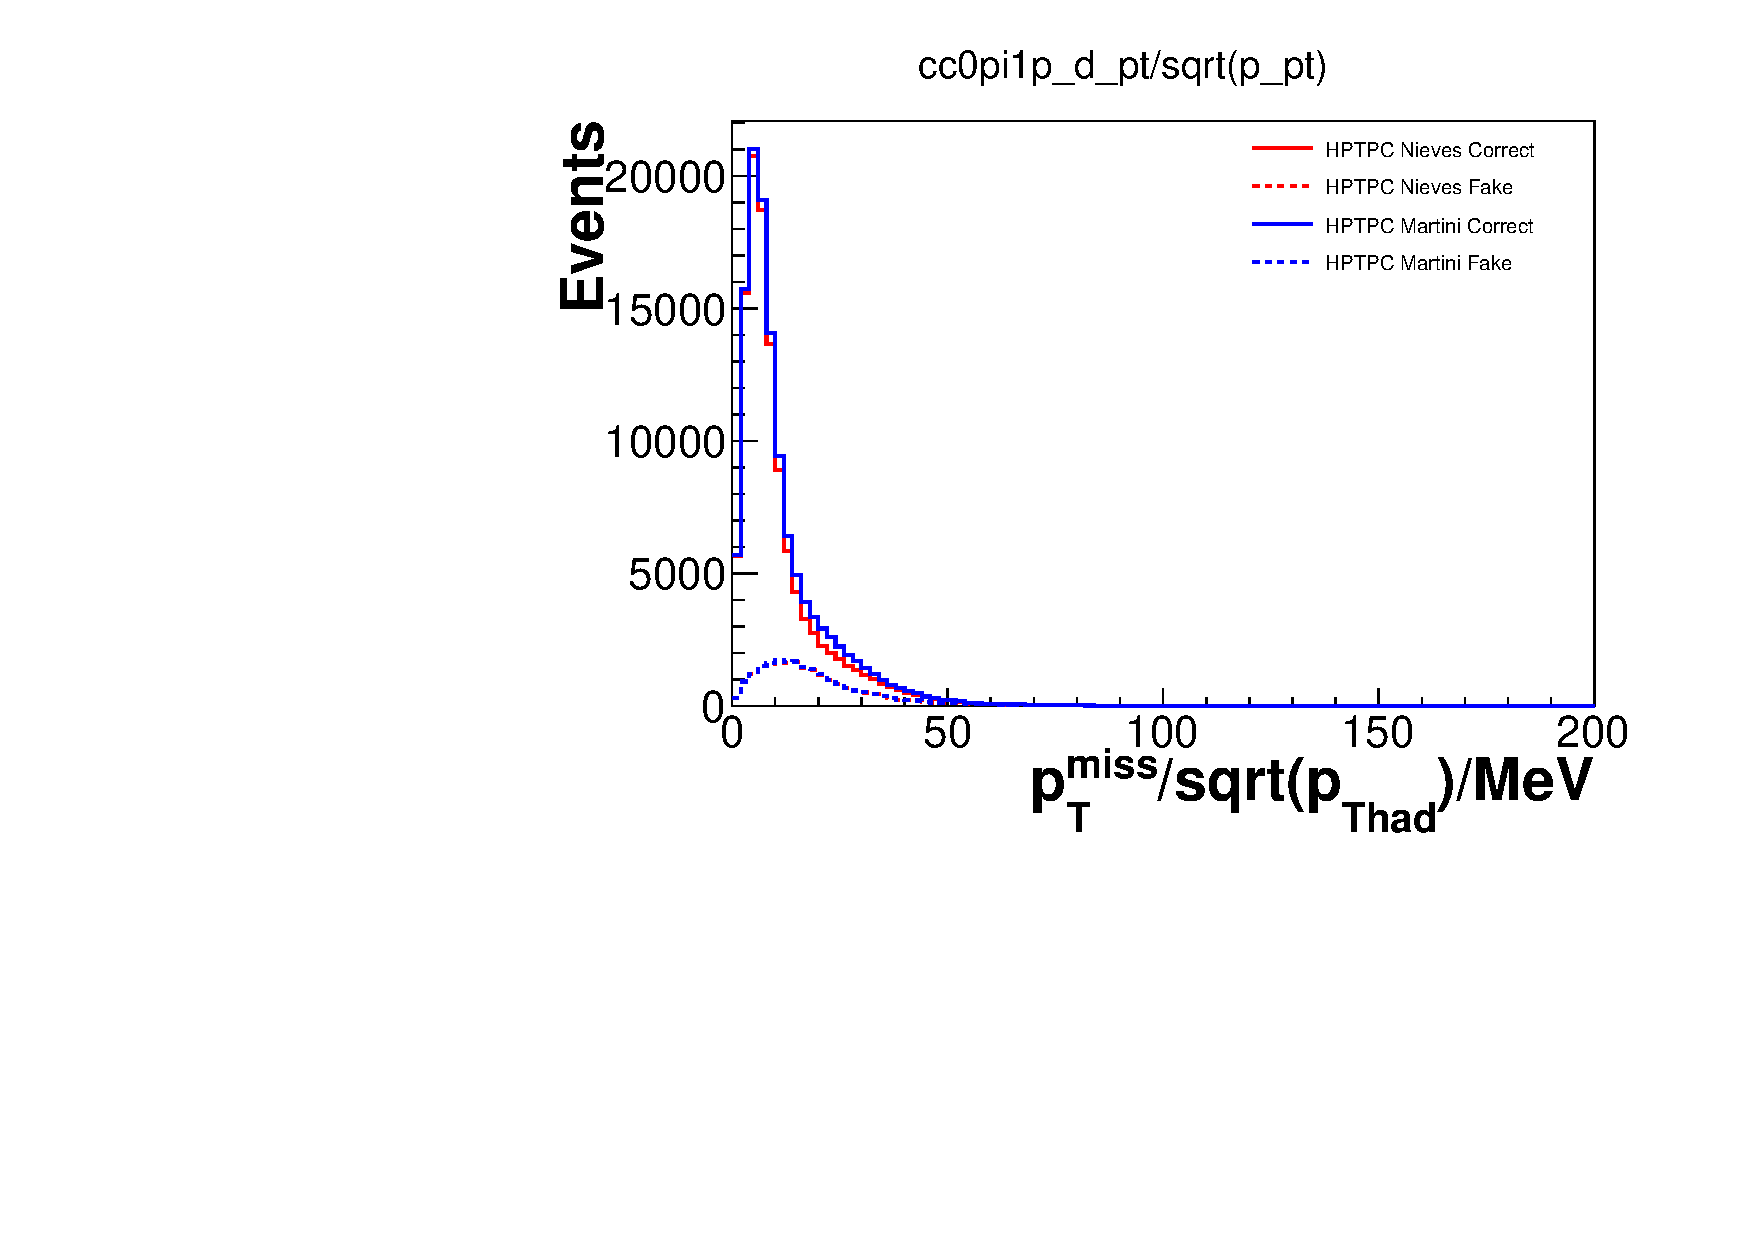
\includegraphics[width=.5\textwidth]{TalkPics/STVforHPTPC_191216/plots_martininieveshptpc/cc0pi1p_metsig.pdf}
  \end{frame}

  \begin{frame}
    \frametitle{CC0$\pi$Np}
    \begin{itemize}
    \item Look at sample with $>=$1 proton and no pions
    \item Expect there may be more power in CC0$\pi$Np because Martini and Nieves predict different proton multiplicities
    \end{itemize}
    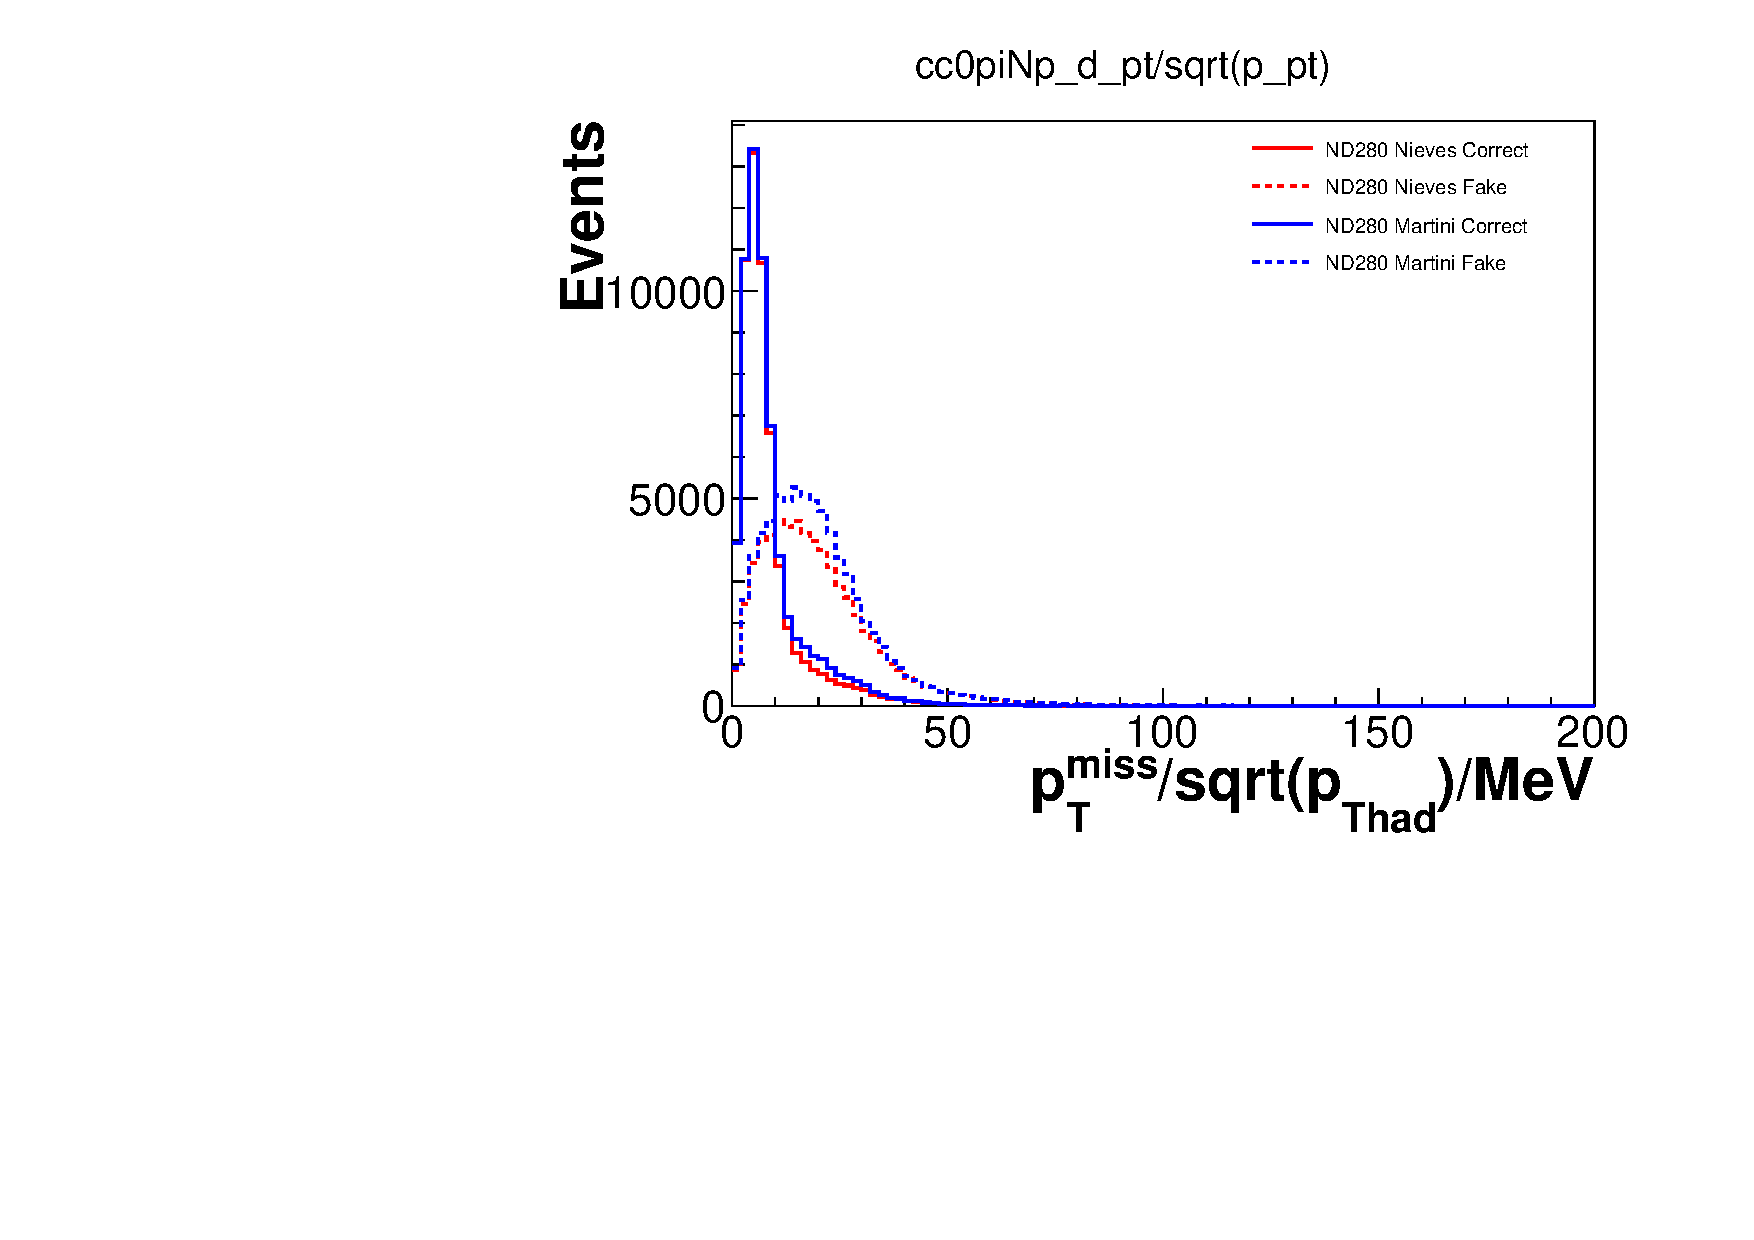
\includegraphics[width=.5\textwidth]{TalkPics/STVforHPTPC_191216/plots_martininievesnd280/cc0piNp_metsig.pdf}
    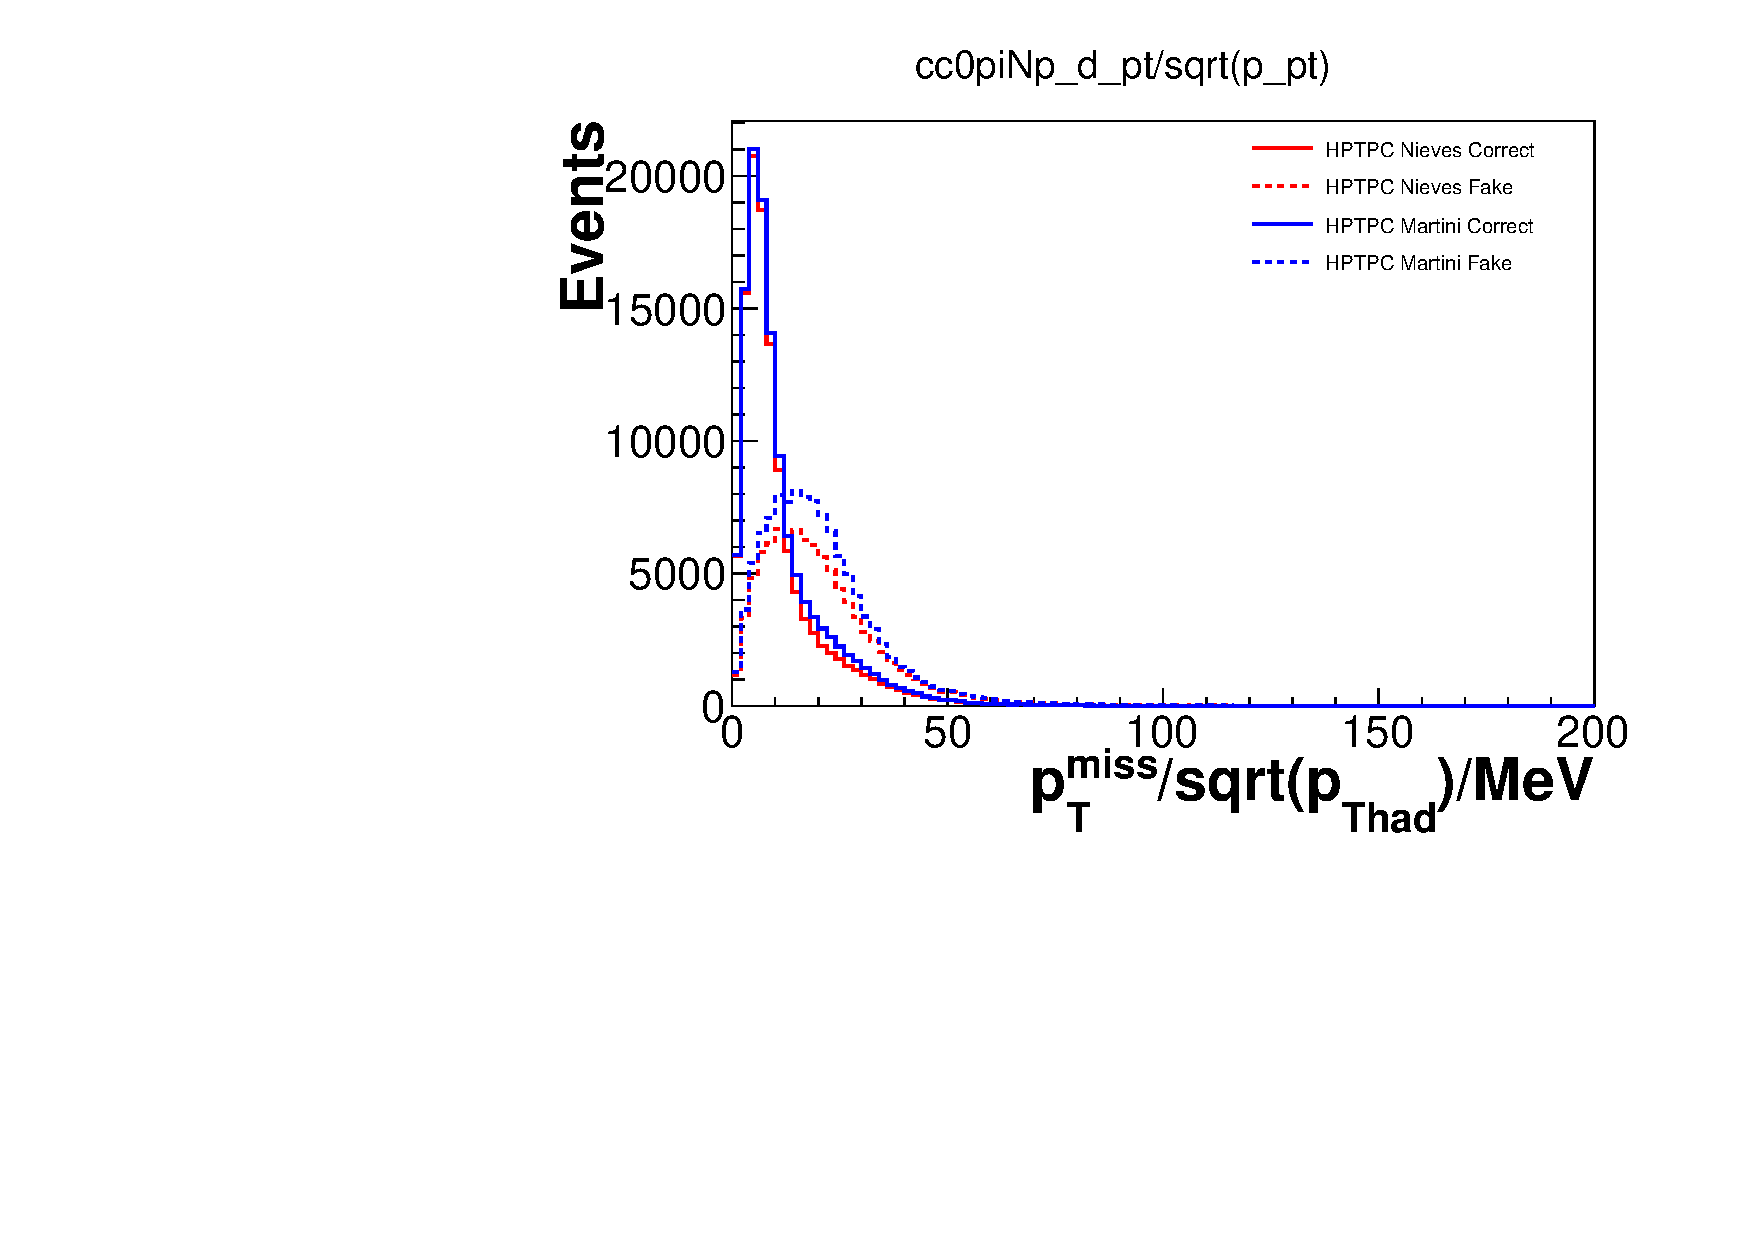
\includegraphics[width=.5\textwidth]{TalkPics/STVforHPTPC_191216/plots_martininieveshptpc/cc0piNp_metsig.pdf}
  \end{frame}

  \begin{frame}
    \frametitle{CC0$\pi$Np}
    \begin{itemize}
    \item Slightly better than CC0$\pi$0p but still not great
    \end{itemize}
    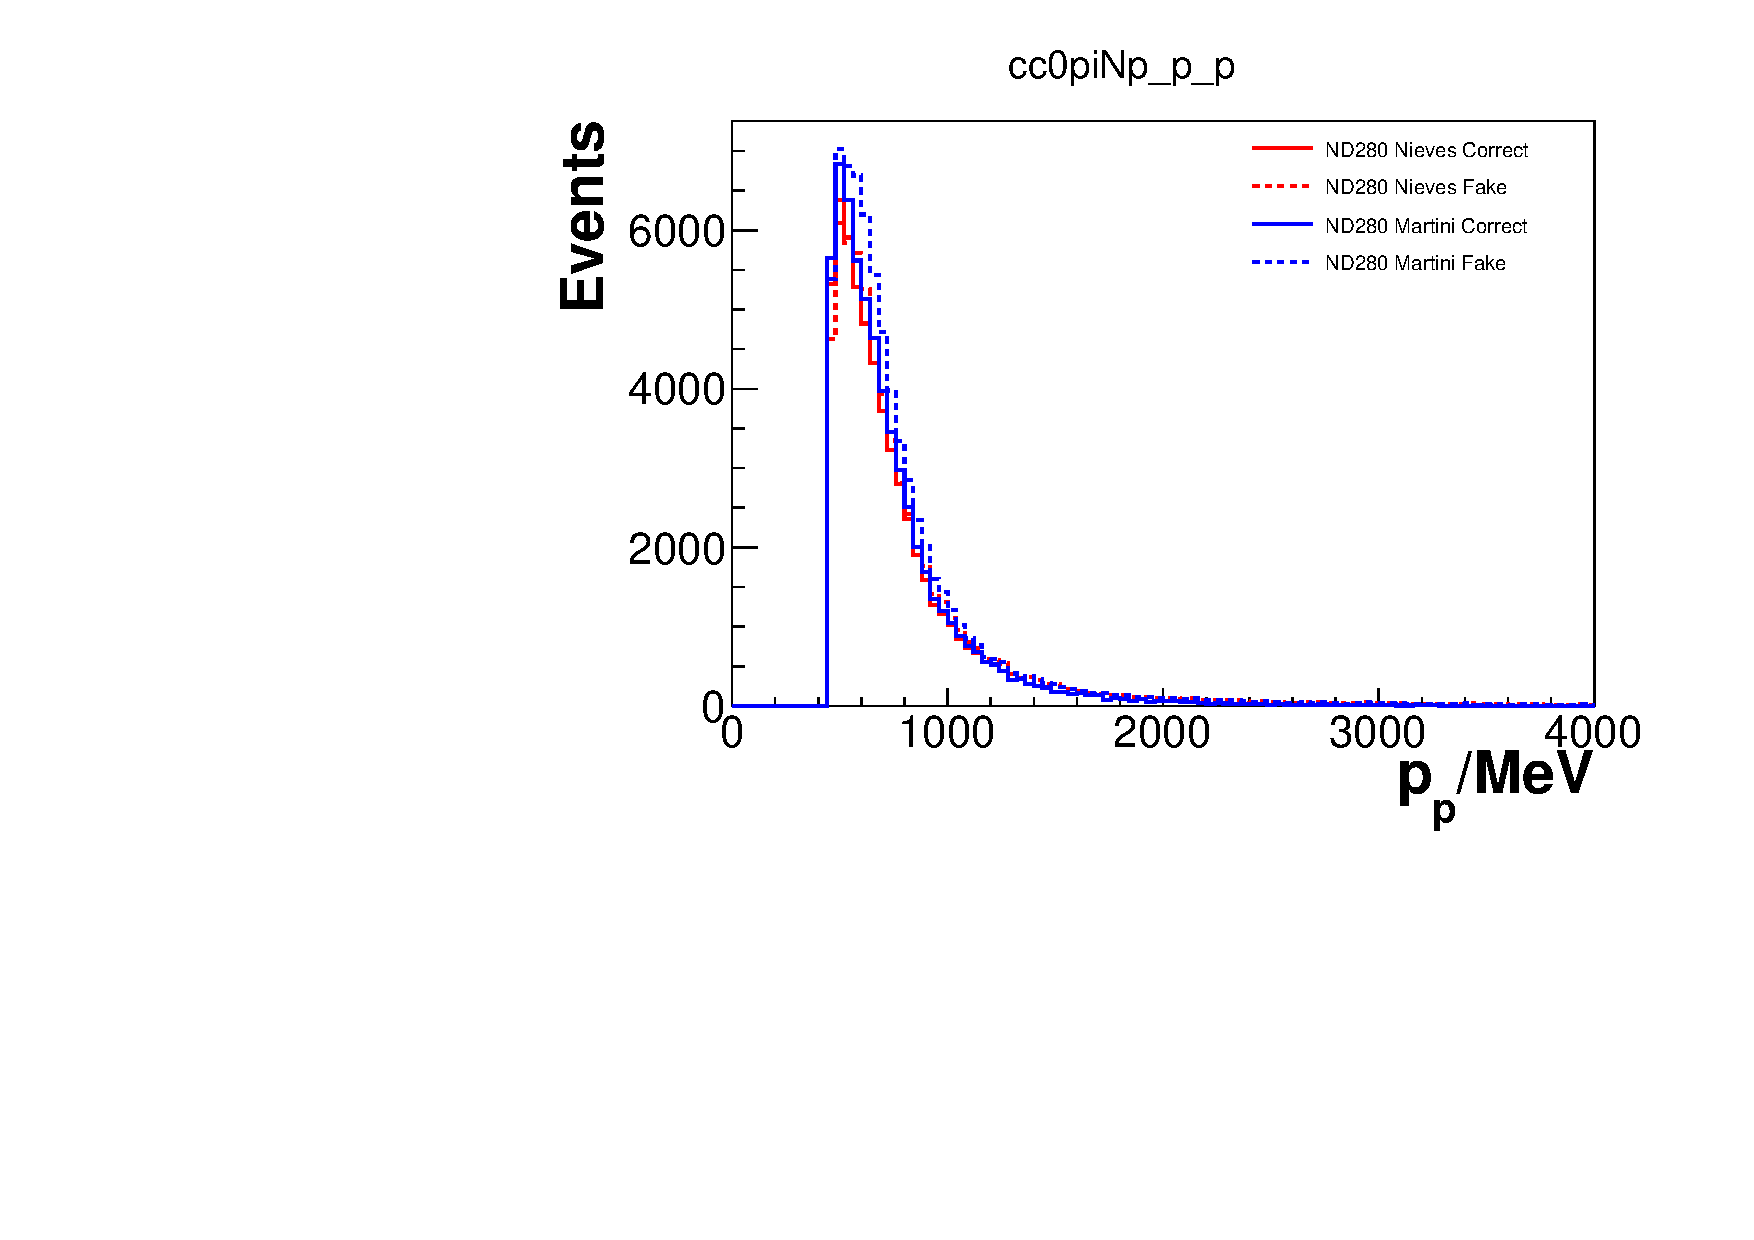
\includegraphics[width=.5\textwidth]{TalkPics/STVforHPTPC_191216/plots_martininievesnd280/cc0piNp_p_p.pdf}
    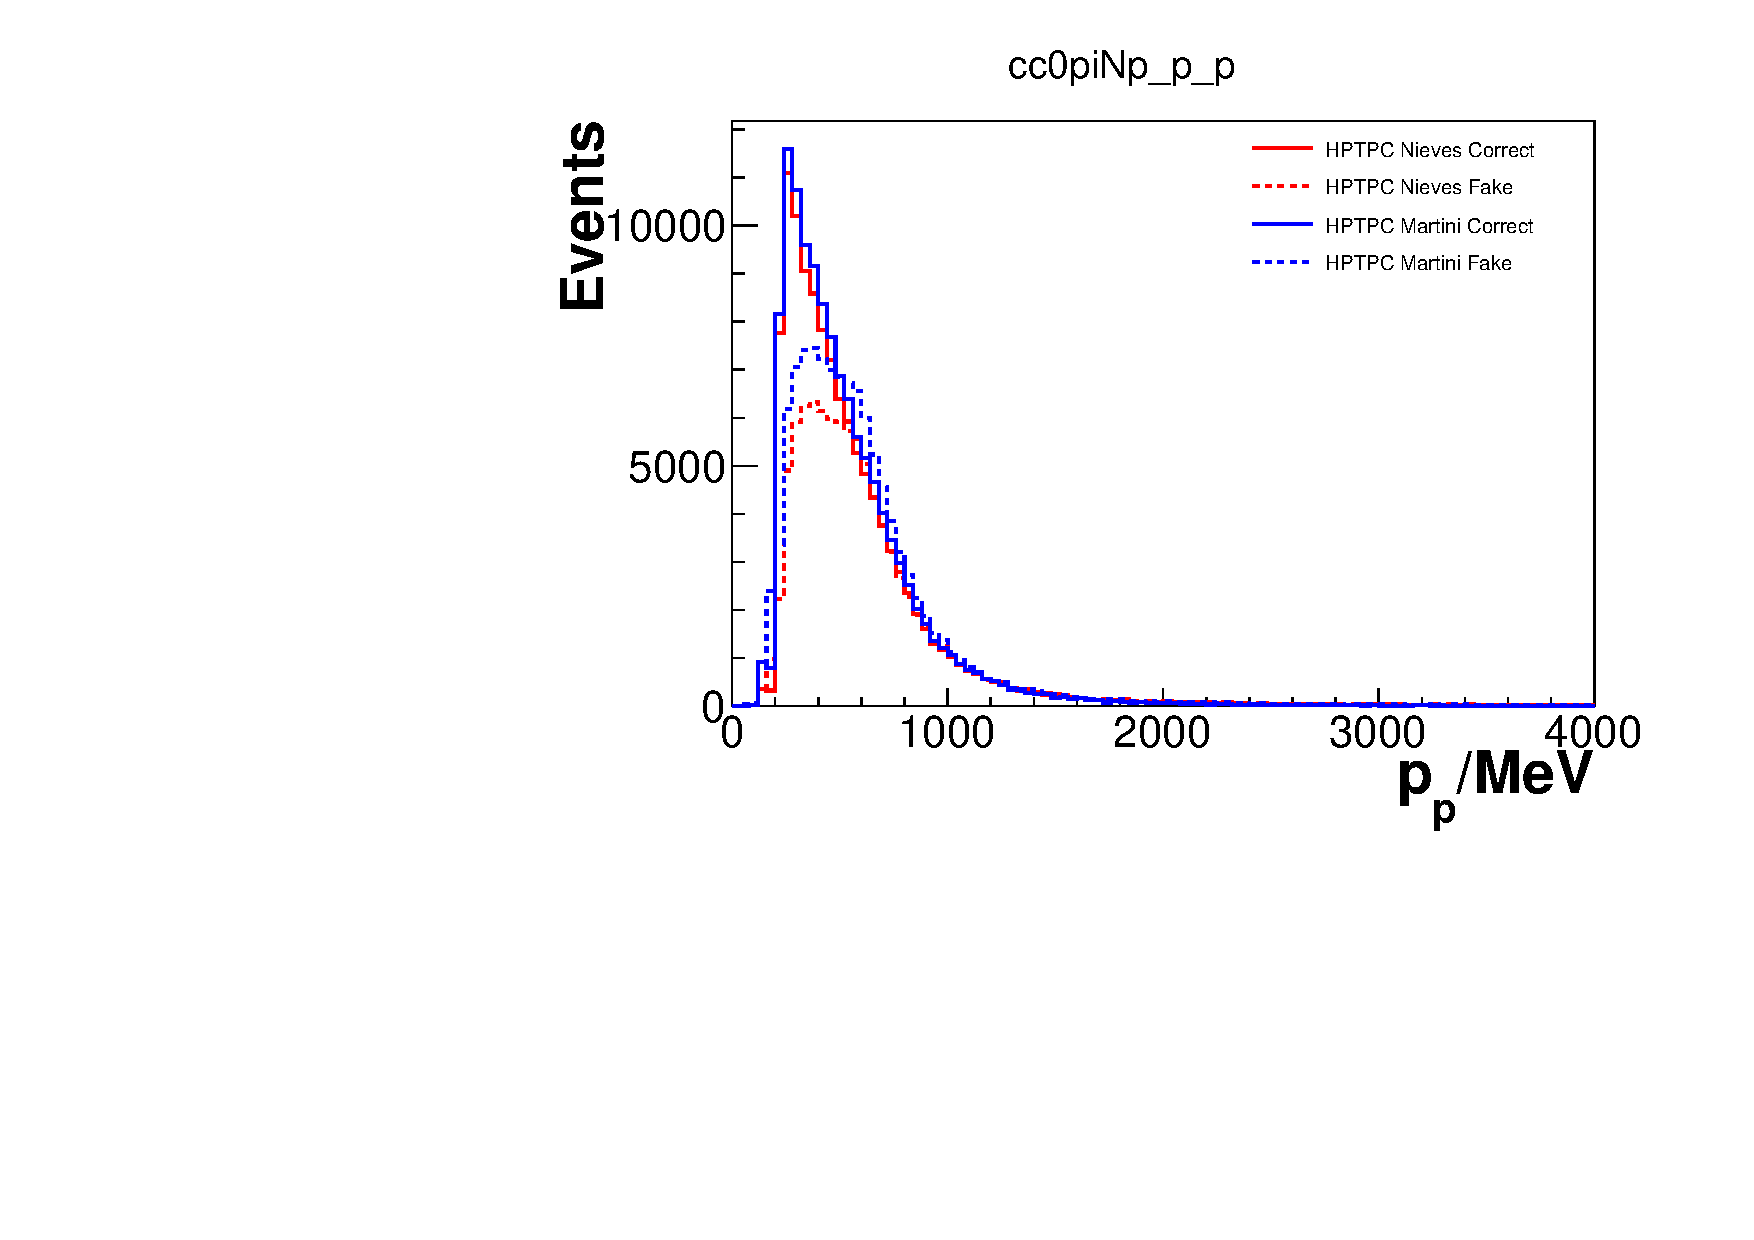
\includegraphics[width=.5\textwidth]{TalkPics/STVforHPTPC_191216/plots_martininieveshptpc/cc0piNp_p_p.pdf}
  \end{frame}

  \begin{frame}
    \frametitle{Why don't we see much model difference?}
    \begin{itemize}
    \item Martini reweighting is done in 1D as a function of $E_{\nu}$
    \item Would not expect this to give a good description of hadronic variables
    \item Solutions:
      \begin{itemize}
      \item[1)] Generate Martini events
      \item[-] Computationally prohibitive
      \item[2)] Come up with a better reweighting scheme
      \item[-] Open to suggestions/help from experts
      \end{itemize}
    \end{itemize}
  \end{frame}

  \begin{frame} 
    \frametitle{HPTPC Hardware R\&D}
    \begin{itemize}
    \item Building 5 Bar, 1$m^3$ prototype HPTPC in UK
    \item Will be being tested in the next year in CERN beam line
    \item Several T2K collaborators involved
    \item Developing full simulation
    \item Looking at reconstruction using T-Rex
    \end{itemize}
    \centering
    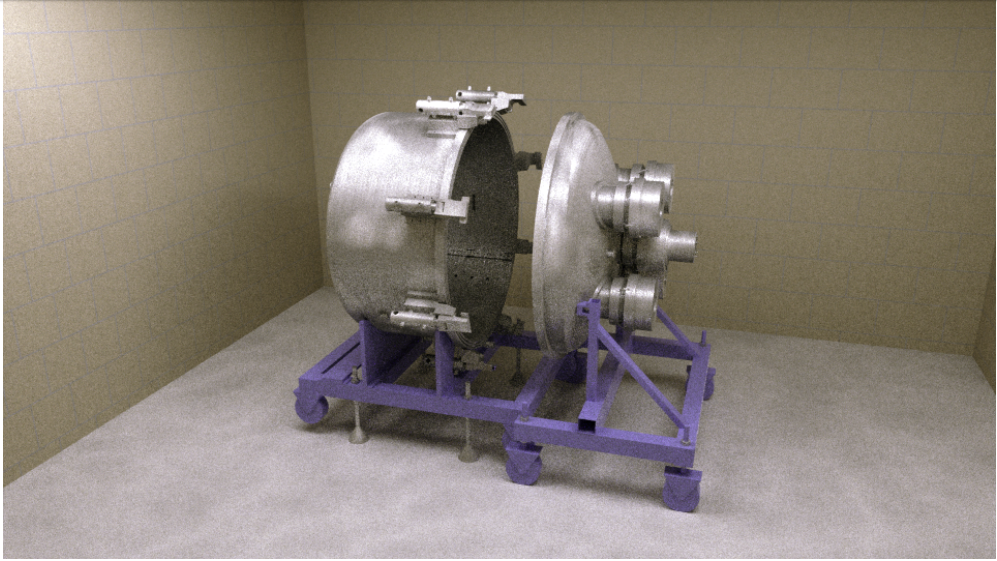
\includegraphics[width=.5\textwidth]{TalkPics/CorrelationWorkshop050217/HPTPCchamber.png}
  \end{frame}

  \begin{frame}
    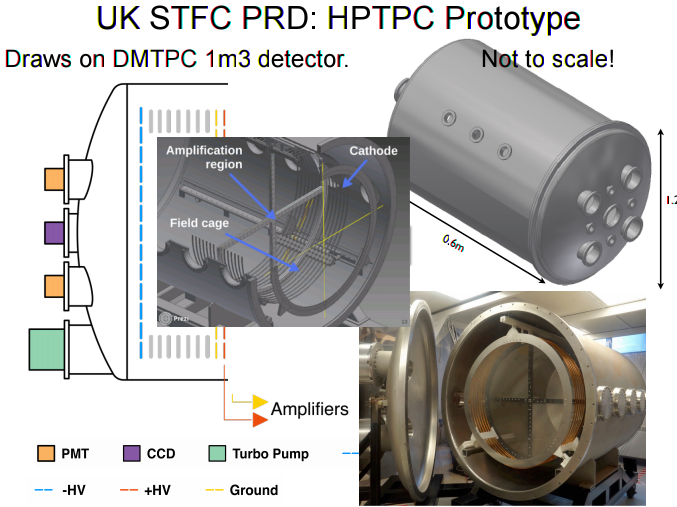
\includegraphics[width=.9\textwidth]{TalkPics/CorrelationWorkshop050217/HPTPCchamber2.png}
  \end{frame}

  
  \begin{frame}
    \frametitle{Conclusions}
    \label{lastframe}
    \begin{block}{}
      \begin{itemize}
      \item HPTPC will have very good hadronic and leptonic momentum thresholds and efficiencies
      \item Will give high purity samples of events to test models with
      \item[-] Full exploitation of this data will need development of model comparison tools
      \item Hardware development well underway with beam tests in the near future
      \item In conjunction with other HK near and intermediate detectors will give much more confidence in our interaction model
      \end{itemize}
    \end{block}
  \end{frame}

  %Backup goes here
  
\end{fmffile}
\end{document}

\begin{frame}
\end{frame}
